\documentclass[10pt]{report}
\usepackage{lingmacros}
\usepackage[normalem]{ulem}
%  Title Formatting 
\usepackage{titlesec}
% Removes paragraph indenting
\usepackage{parskip} 

% Figure labeling
\usepackage{hyperref}

\usepackage{amsmath}

% Font
\usepackage{tgpagella}

% Inline code
\usepackage{listings, lstautogobble, newtxtt}
\lstset{basicstyle=\ttfamily, keywordstyle=\bfseries}

\usepackage[labelfont=bf, labelsep=period]{caption}
\usepackage{graphicx}
\graphicspath{ {./images/} }

% Makes citations superscript
\usepackage[superscript,biblabel]{cite}
\usepackage{url}
\urlstyle{same}

\lstset{aboveskip=20pt,belowskip=20pt}

\titleformat{\chapter}[block]
{\normalfont\huge\bfseries}{\thechapter.}{1em}{\Huge}
\titlespacing*{\chapter}{0pt}{-19pt}{0pt}

\lstset{language=Java,
	showstringspaces=false,
	breaklines=true,
	frameround=ffff,
	frame=single,
	autogobble=true
}

\renewcommand{\subsectionautorefname}{section}


\begin{document}
	\begin{titlepage}
		\begin{center}
			\Large
			\textbf{Procedural Content Generation Using Noise}
			
			\vspace{1.5cm}
			\normalsize
			\textbf{Michael Li}
			
			\vfill
			
			\textbf{DRAFT 4.5.1}
			
			\uline{Dianne Hansford, Ph.D \hfill Director}
			\vspace{1cm}
			
			\uline{Yoshihiro Kobayashi, Ph.D \hfill Second Committee Member}
			
			\vspace{3cm}
			
			
\includegraphics[scale=.5]{asu_barretthonors_horiz_rgb_maroongold_600ppi}
			
			\vspace{1.5cm}
			Ira A. Fulton Schools of Engineering
			
			School of Computing, Informatics, and Decision Systems Engineering
			
			Spring 2021
			
		\end{center}
	\end{titlepage}
	
	\chapter*{Abstract}
	
	\addcontentsline{toc}{chapter}{Abstract}
	Procedural content generation refers to the creation of data algorithmically using controlled randomness. These algorithms can be used to generate complex environments as opposed to manually creating environments, using photogrammetry, or other means. Procedurally generated content can be created using noise based algorithms. This paper will detail procedural generation of content using noise.
	
	\clearpage
	
	\tableofcontents
	
	\clearpage
	
	\let\clearpage\relax
	\chapter{Introduction}
		
		Procedurally generated content is an often hidden, yet common feature among digital content, as it automates the creation of large amounts of data. Often, this is hidden in the backgrounds of movies and video games, as well as other art -- adding subtle texture and variation. \emph{Procedural content generation} (PCG) has many possible outputs, with some examples being the generation of stories, histories, particle effects, and characters. PCG refers to the use of computers to algorithmically create data using a pseudo-random procedural algorithm, which is then interpreted into content. One of the most famous cases of PCG is Minecraft \cite{minecraft-gen}, generating geological formations and terrain. A \emph{geological formation}, is a body of rock that possesses some degree of internal consistency or distinctive features \cite{2005}. This allows geological formations to be separate from the region it is placed in while still being a landmark for the region as a whole. Just as sand is individually different at a small scale, so too is the data created by procedural generation. However, when viewed as a whole, there is little difference between each grain. This necessitates user control and adjustments in order to make a region stand out versus another, with the use of landmarks or geological formations. Other examples of procedural generation's varied uses include games such as The Elder Scrolls II: Daggerfall, which employs various forms of procedural generation to determine the location of non-player characters, the layout of dungeons, as well as the terrain itself \cite{daggerfall}. In more complex cases, procedural generation is used to create fake histories, with the more well-known example of Dwarf Fortress \cite{df-dev}. However, procedural generation's applications are not only limited to games. In The Lord of the Rings, many of the scenes with large amounts of characters were created using procedural generation, ensuring individual animations of the slightly differentiated characters \cite{massive}.
		
		This paper explains procedural algorithms involving noise, and noise's application in generating geological formations and the surrounding terrain. A procedural algorithm for producing noise returns a value in the range of \([0,1]\). For this paper, the process of Perlin noise and its derivatives will be focused on. Some other examples of procedural algorithms to create content include noise, fractals, as well as cellular automata. These algorithms can be mixed and matched in any number of ways to fine-tune different outcomes, or to add variety to content. To qualify as PCG, the algorithm to create data must be modifiable and controllable, while the results from the algorithm must be reproducible. The reproducible criteria for PCG can be fulfilled by the use of deterministic random number generators (see \autoref{subsec:rng}), but some forms of procedural algorithms are majority governed by randomness. The modifiable criteria is fulfilled by the use of parameters to modify the algorithm. A deterministic system is a system in which no randomness is involved, while a stochastic system is one that can be described by a random probability distribution. While these concepts may seem to be mutually exclusive, they occupy different portions of the overall procedural generation pipeline, allowing them to co-exist. 
		
		\subsection{It's Not All About Noise}
		
		While noise is the focus of this paper, it is important to note that there are alternatives to noise for PCG. Here we provide two alternatives to noise for PCG: fractals and cellular automata. In \autoref{chap:development}, the history of these alternatives, and some of their relations to the development of noise will be briefly explored. 
		
		Fractal-based algorithms utilize the mathematics of fractals for the purpose of PCG. \emph{Fractals} are characterized by their self-similarity. This means that the parts of the whole fractal contain the same characteristics. One example of this is the Koch snowflake. The Koch snowflake's rule, described in \autoref{enum:koch}, is fairly simple. However, by just replacing each line segment with a line segment with a triangular portion jutting out, \autoref{fig:m_koch} is the result.
		
		\begin{enumerate} \label{enum:koch}
			\item Draw an Equilateral triangle
			\item Replace all lines as follows, and repeat 2
		\end{enumerate}
		
		\begin{minipage}{\textwidth}
			\centering
			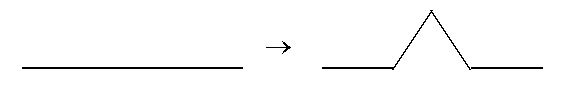
\includegraphics[scale=0.5]{m_reprule}
			\captionof{figure}{Rule of the Koch snowflake \cite{fractal-landscapes}.}
			\label{fig:m_reprule}
		\end{minipage}
		
		\begin{minipage}{\textwidth}
			\centering
			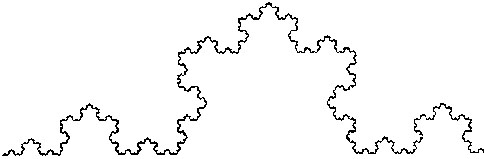
\includegraphics[scale=0.5]{m_koch}
			\captionof{figure}{Koch snowflake \cite{fractal-landscapes}.}
			\label{fig:m_koch}
		\end{minipage}
	
		The rule described for the creation of the Koch snowflake can be repeated endlessly. Fractals and the subsequent geometric shapes that can be created from fractals were found to be useful in describing nature. By studying geographical data, many similarities such as self-similarity and the subdivision of space were found, pushing the study of fractal geometry forward \cite{doi:10.1111/j.1467-8306.1987.tb00158.x}. 
		
		Another method of generating terrain and other features such as caves \cite{10.1145/1814256.1814266} revolves around the use of cellular automata. Cellular automata are a model of a system of cell objects with three characteristics. The cells must be placed on a regularly spaced grid, regardless of dimensionality. These cells must each have a state, which can describe any number of features for each individual cell. Lastly, each cell must have a neighborhood. While typically a neighborhood is composed of only the adjacent cells, it can be defined in any number of ways. This approach relies on having the information of neighbors and the states of their neighbors to determine surrounding cells to then modify their states \cite{nature-of-code}. In \autoref{fig:cell-30}, each row of the graph shows an iteration of the algorithm. Each cell has two states, either black or white, and their neighbor the cells on both sides. This particular cellular automaton has seven rules, shown at the bottom of the figure. 
		
		\begin{minipage}{\textwidth}
			\centering
			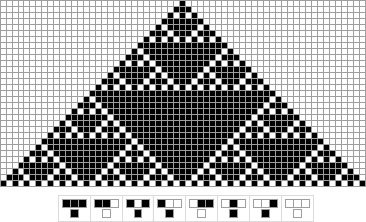
\includegraphics[scale=0.7]{rule-30}
			\captionof{figure}{1-Dimensional cellular automata example. Each row is an iteration, following the eight rules at the bottom \cite{cell-30}.}
			\label{fig:cell-30}
		\end{minipage}
		
		\begin{minipage}{\textwidth}
			\centering
			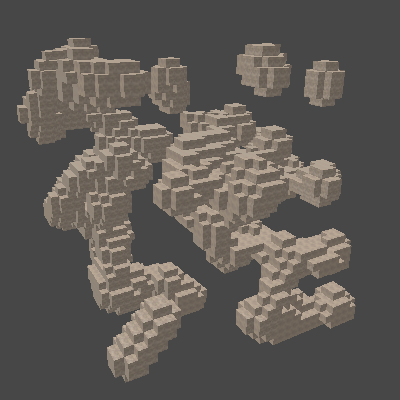
\includegraphics[scale=.6]{cellular-automata-cave}
			\captionof{figure}{An example of three-dimensional cellular automata cave generation \cite{bergauer_prozedurale_nodate}}
			\label{fig:ca-cave}
		\end{minipage}
		
		\section{Motivation for Procedurally Generated Content}
		
		\emph{Topography} is the study of the land surface, encompassing both natural and artificial features covering the surface. Procedural content generation is often used in the creation of features such as geological formations and topography due to the self-similarity found in nature. While fractals serve as a good description of the self-similar properties of edge-like features, as well as edge measurement issues \cite{ijgi5060095}, noise can also generate these features, as well as filling out the areas in between more easily than fractal algorithms. While creating these features is possible through other means, such as by hand or through photogrammetric methods \cite{bullinger2020photogrammetrybased}, using procedural algorithms allows for easier control over much larger surfaces, and can lead to similar quality results with the reduction of manual labor. This allows for smaller teams to more easily populate and create densely featured worlds. Some examples of this can be found in the procedural coverage and generation of vegetation of terrain, respectively, using custom built tools \cite{redengine}, or tools such as World Machine \cite{world-machine}. Another common example of procedural generation is hidden in the backgrounds of movies, with procedural algorithms populating the topography in Pixar movies \cite{10.1145/3388767.3407372}. These often unnoticed, or glazed over details prove a challenging problem. Creating something from nothing, and arranging randomly generated data takes a lot of processing, steps, and subjective decisions.
		
		\section{Fundamentals} % true random number table
			\subsection{Random Numbers} \label{subsec:rng}
		
			A foundational concept of all PCG is the creation random numbers. The generation of random numbers is difficult as the algorithm or process used to obtain random numbers must not output random numbers with any recognizable patterns or regularities. This property is know as \emph{statistical randomness}. Statistical randomness ensures that the probability distribution is uniform, with any number in the given range having an equal chance of being selected. Random numbers may be generated \emph{non-deterministically} through the interpretation of unpredictable physical processes, and \emph{deterministically} using an algorithm \cite{rng}. These methods are also known as random bit generators, \emph{Non-deterministic Random Bit Generators} (NRBG) and \emph{Deterministic Random Bit Generators} (DRBG), respectively. One example of an unpredictable physical process to generate non-deterministic random numbers is through using radio receivers to pick up atmospheric noise \cite{random-org}. A NRBG measures a random physical process such as atmospheric noise and compensates for potential biases to generate a random number. While it is "theoretically impossible to prove that a random number generator is really random," the numbers produced by the generator can be analyzed to increase or decrease confidence in the generator \cite{random-org}. For deterministically generated random numbers the random numbers are algorithmically determined using an input value, also known as a \emph{seed}. A DRBG is an algorithm to generate a sequence of numbers whose distribution approximates a sequence of random numbers. The algorithm to create these numbers is \emph{static}, or unchanging -- by inputting a seed, the same sequence of random numbers will always be created. This property of seeding differentiates a DRBG and a NRBG. While a DRBG's outputs are not truly random, the output values in the long term should approximate a NRBG's results.  
			
			The concept of reproducibility is shared between PCG and DRBG's. DRBG's are also known as pseudo-random number generators since the generated numbers from DRBG's are described as pseudo-random because they only approximate randomness \cite{rng}. This is due to the necessity of the seeding value, ensuring the deterministic portion of the definition. PCG follows the same methodology as DRBGs. PCG often uses a seed for the procedural algorithm. While not all procedural generation uses a seeding function, seeding is a common property among PCG. In procedural algorithms, an input seed ensures the reproducibility, regularity as well as controlled randomness. By using a seed to determine the initial state of the DRBG, the sequence of random numbers is fixed for use by the procedural algorithm. An example of DRBG is shown in \autoref{lst:np.random}, using NumPy \footnote{NumPy is a math library for Python. Functions from this library will have a preceding "np."}.
			
			\begin{lstlisting}[label={lst:np.random}, language=Python, frame=none, caption={An example of seeding NumPy's random function in Python.}, captionpos=b]				
				np.random.seed(10)
				np.random.rand(5)
			\end{lstlisting}
			
			For example, in \autoref{lst:np.random}, the same five digits 
			
			$$ \begin{matrix}
				0.77132064 & 
				0.02075195 & 
				0.63364823 & 
				0.74880388 & 
				0.49850701
			\end{matrix} $$
			
			will always be returned, in the same order order, because of the use of 10 as the seed for the DRBG. In Python, there are no differences between float and double types. Float is a data-type built into Python, while the double data-type, which are what this function returns, come from NumPy.
			
			\subsection{Interpolation} \label{subsec:interpolation}
			
			In addition to random numbers, interpolation is another concept integral to noise. \emph{Interpolation} estimates the value between two points. For example, using linear interpolation and given the two points (1,1) and (3,3), the assumption would be a constant slope between these two points. 
			
			\begin{minipage}{\textwidth}
				\centering
				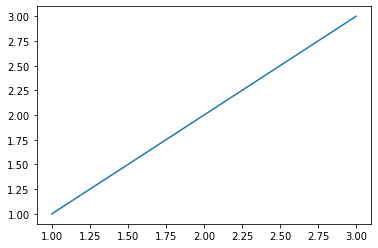
\includegraphics[scale=.5]{linear-interpolation}
				\captionof{figure}{Plot of the two points (1,1) and (3,3), as well as a linear function between the two.}
				\label{fig:linear-interpolation}
			\end{minipage}
			
			If asked to estimate the y-value of \(x = 2\), for linear interpolation, two other points are needed. For example, if \((x_0,y_0) = (1,1)\), and \((x_1,y_1) = (3,3)\) the result would be \(2\), due to the linear interpolation formula
			
			\[y = \frac{y_0 (x_1 - x) + y_1 (x - x_0)}{(x_1 - x_0)}\].
			
			This linear interpolation function can also be implemented in code. However, this function will not work if the two known points have the same value as there will be a divide by zero error. An alternate method of calculating linear interpolation, known as the \lstinline|lerp| function, can be used instead. The \lstinline|lerp| function uses the ratio of the distance between points to calculate the estimated value. Instead of calculating for a point, the ratio of the distances between the two known points is needed. Using the same \((x_0,y_0)\) and \((x_1,y_1)\) points, to calculate a point in the middle of the two, two \lstinline|lerp| operations are required. Since the target point is in the middle of the two values, the target point's distance between the two knowns is the same, giving \(t_0 = t_1 = 0.5\). First, \lstinline|lerp(t_0, x_0, x_1)| gives the \(x\)-value, then \lstinline|lerp(t_0, y_0, y_1)| gives the \(y\)-value.
			
			\begin{lstlisting}[label={lst:lerp}, language=Python, frame=none, caption={lerp function in Python.}, captionpos=b]
				def lerp(t, a, b):
					return a + t * (b - a)
			\end{lstlisting}
			
			Linear interpolation is not the only form of interpolation. Two other forms of interpolation commonly used for Perlin noise include cosine interpolation as well as smooth-step interpolation. Smooth-step interpolation instead estimates the target value according to a signmoid-like function, shown in \autoref{fig:smoo}.
			
			\begin{minipage}{\textwidth}
				\centering
				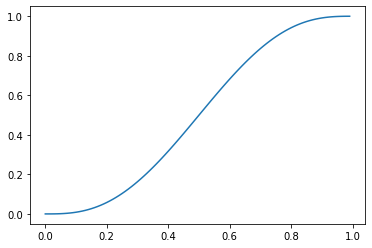
\includegraphics[scale=.5]{smooth}
				\captionof{figure}{Example of a sigmoid-like function using smooth-step interpolation. Note the differences compared to the result of \autoref{fig:linear-interpolation}}
				\label{fig:smoo}
			\end{minipage}
			
			The suggested formula by Perlin for this interpolation was \(3t^2 - 2t^3\), but has since been superseded. One of the problems with the previous equation used was that the second derivative of the function, \(6-12t\) is not zero at either \lstinline|t=0| or \lstinline|t=1|, causing discontinuities in the noise. This led the improved equation, shown in \autoref{eq:smooth}\cite{10.1145/566654.566636}. 
			
			\begin{equation} \label{eq:smooth}
				t = 6t^5 - 15t^4 - 10t^3
			\end{equation}
		
			\begin{lstlisting}[label={lst:fadee}, language=Python, frame=none, caption={Smooth-step interpolation implementation, suggested by Perlin.}, captionpos=b]
				def fade(t):
					return t * t * t * (t * (t * 6 - 15) + 10)
			\end{lstlisting}
			
			This function and the original differ in that the newer, higher order function has a zero second derivative at the endpoints, giving it a continuous second derivative everywhere \cite{simplex-demyst}. For example, using lerp and the values \((x_0,y_0) = (0,0)\), and \((x_1,y_1) = (1,1)\), and a distance of \(0.9\), the result would be \((t_0, t_1) = (0.9, 0.9)\). However, using smoothstep interpolation, \((0.99, 0.99)\).
			
			Interpolation's goal is to address \emph{visual artifacting} or \emph{artifacting} in the result of noise algorithms. Visual artifacting refers to anomalies or errors in a visual representation. Since noise is entirely composed of these artifacts, it seems a little counter-intuitive, but the goal of PCG and procedural algorithms is to have controlled randomness. In \autoref{fig:pnartifact}, straight lines can be seen throughout the pattern appearing on the surface of the cube. These irregularities to the smoothed pattern of the cube are artifacts in this context -- they are not the intended result of the procedural algorithm.
			
	\vspace{10pt}
	\let\clearpage\relax
	\chapter{Noise}
		
		Perlin noise (introduced in \autoref{sec:1d}) and Simplex noise (introduced in \autoref{sec:n-dim}) are examples of gradient noises, which are based around lattices. A \emph{lattice} is a regularly spaced array of points \cite{integer-lattice}. In one dimension, this appears as a number line. 
		
		\begin{minipage}{\textwidth}
			\centering
			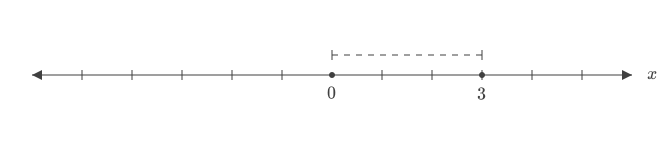
\includegraphics[scale=.4]{1d}
			\captionof{figure}{One-dimensional integer lattice \cite{cartesian}}
			\label{fig:1d}
		\end{minipage}
	
		In two dimensions, this becomes a Cartesian coordinate plane in two dimensions, an array of squares.
	
		\begin{minipage}{\textwidth}
			\centering
			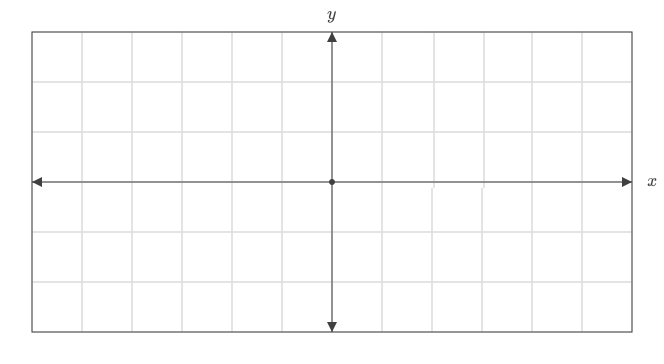
\includegraphics[scale=.35]{2d}
			\captionof{figure}{Two-dimensional integer lattice \cite{cartesian}}
			\label{fig:2d}
		\end{minipage}
	
		In three dimensions, this becomes a Cartesian coordinate system in three dimensions, an array of cubes.
		
		\begin{minipage}{\textwidth}
			\centering
			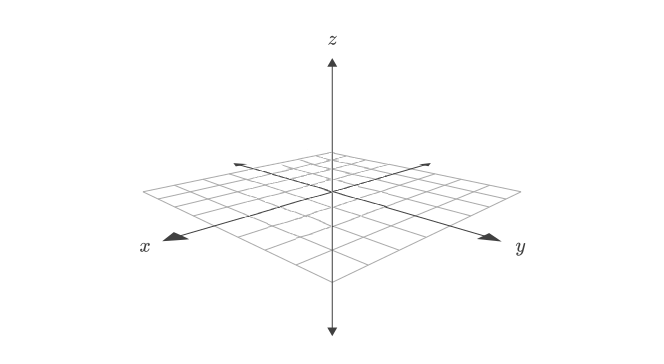
\includegraphics[scale=.5]{3d}
			\captionof{figure}{Three-dimensional integer lattice \cite{cartesian}}
			\label{fig:3d}
		\end{minipage}
	
		The dimensionality of Perlin noise can extend to n-dimensions. For lattices used to generate noise, the spacing of points is most commonly found as integer points to save on computational and memory resources. These lattices form the basis of Perlin noise. For a Perlin noise function, first a method of creating storing a pseudo-random gradient vector at each lattice point is required. This can be accomplished through seeding a DRBG, or by using a hashing function (see \autoref{subsec:hashing}). These algorithms use a seed to produce this set of pseudo-random gradients, although this seed number will only have meaning in the context of the same algorithm it is being used in -- changing the algorithms and/or manipulating the seed will change the entire output, so reproducibility limited to a per-version context. Then, the goal is to interpolate the gradient values between these lattice points, to smoothly transition from one to another. 
		
		
		% https://stackoverflow.com/questions/10729891/perlin-noise-gradient-function Literally a godsend
		\subsection{Hashing} \label{subsec:hashing}
			Perlin's noise implements a hash function instead of using a an array of values produced by a DRBG \cite{improv-noise}. A \emph{hash table} maps a \emph{key} (input) to a unique \emph{bucket} (output), in an array of buckets, through the use of a hash function. This hash function compute the index of a bucket from the key. Since  This both serves as an efficient storage method, as each random number needed can be algorithmically determined from the coordinate point, as well as allowing for memory constraints to be lowered, due to the need for just a hashing function. Perlin's hashing function consists of the set of integers in \([0, 255]\), stored in an array \lstinline|p[]|, ordered randomly. 
			
			\begin{lstlisting}[language=Python, frame=none, caption={Unit cube's corner minimum values}, captionpos=b]
				...
				x_min = int(x)
				x_max = x_min + 1
				
				y_min = int(y)
				y_max = y_min + 1
				
				z_min = int(z)
				z_max = z_min + 1
				...
			\end{lstlisting}
			
			To calculate the random value needed for a given \((x,y,z)\) point, eight values are needed for the unit cube surrounding the point. First, the value of the minimum and the maximum bound of the unit cube in the x dimension must be hashed. 
			
			\begin{lstlisting}[label={lst:hashx}, language=Python, frame=none]
				A = p[x_min]
				B = p[x_max]
			\end{lstlisting}
			
			Then, the value of the minimum and the maximum bound of the unit cube in the y dimension will each be added to each of these hash values, resulting in four total values. 
			
			\begin{lstlisting}[label={lst:hashx}, language=Python, frame=none]
				AA = p[A + y_min]
				BA = p[B + y_min]
				
				AB = p[A + y_max]
				BB = p[B + y_max]
			\end{lstlisting}
			
			Lastly, the minimum and the maximum bound of the unit cube in the z dimension will each be added to each of these hash values, resulting in eight total values -- one for each corner of the unit cube. 
			
			\begin{lstlisting}[label={lst:hashx}, language=Python, frame=none]
				AAA = p[AA + z_min]
				AAB = p[AA + z_max]
				
				BAA = p[BA + z_min]
				BAB = p[BA + z_max]
				
				ABA = p[AB + z_min]
				ABB = p[AB + z_max]
				
				BBA = p[BB + z_min]
				BBB = p[BB + z_max]
			\end{lstlisting}
		
			This pseudo-randomly generates values that are reverse calculatable, given the same hash table. In this sense, the hash table can act as a seed for the Perlin noise algorithm as well. 
	
		\section{1-Dimensional Perlin Noise} \label{sec:1d}
		
			For one-dimensional Perlin noise, the associated lattice will be a number line. At each of the integer \((x,y)\) coordinates, a pseudo-random one-dimensional vector in the range of \([0,1]\) is generated. These vectors can either be generated at run-time through a DRBG (introduced in more detail in \autoref{subsec:hashing}), or be stored beforehand. In this example, these vectors are being stored in an array. This value represents a gradient, or a slope, at each of the integer coordinates. This gives Perlin noise the category of gradient noise, as opposed to if the values were simply interpreted as values, as in value noise. For simplicity, this pseudo-random gradient value will be represented by \(y\). In one dimension, gradients are one dimensional as well. The goal is to determine the one-dimensional \(y\) vector at a coordinate, or set of coordinates, at a \(x\) coordinate. 
			
			The influence of the gradient value of each of the surrounding integer coordinates must be found based on the distance from the point in question. The closer the surrounding coordinate, the larger of an effect the coordinate will have on the final value. In one dimension, there will be two of these \emph{influence values}. In \autoref{fig:lower_upper}, the surrounding coordinates are pictured in red, and the point in question is pictured in blue. These two influence values can be determined by the distance vector from each coordinate, multiplied by the gradient value at each point. 
			
			\begin{minipage}{\textwidth}
				\centering
				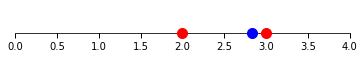
\includegraphics[scale=0.75]{lower_upper}
				\captionof{figure}{The lower and upper integer bounds for an arbitrary input.}
				\label{fig:lower_upper}
			\end{minipage}
			
			The two points in red must be found first. To do this, round the input \(x\). This will give one of the surrounding values. To get the other value, subtract one if the value was rounded down, otherwise add one. This process is demonstrated in \autoref{lst:minmax}, where the input, x, is a floating point number. Using a floor,ceiling, or casting x as an integer will accomplish the same thing as rounding. The, since this will always round down, the other value is found by adding one. 
			
			\begin{lstlisting}[label={lst:minmax}, language=Python, frame=none, caption={An example of finding the min bounds in 1D Perlin noise, given input x. This implementation uses a floor function to calculate the minimum value, and an \lstinline|& 255| operation to ensure the X distance is eight-bits. This will be used in two and three dimensional implementations, for the hashing system.}, captionpos=b]
				X = int(math.floor(x)) & 255
			\end{lstlisting}
		
			Vectors from the input coordinate to the two neighboring integer coordinates can then be calculated by subtracting each integer coordinate from the input \(x\) value. This gives a distance vector (which is one-dimensional in this case). This distance calculation is shown in \autoref{lst:dst}, giving us \lstinline|x|. 
		
			\begin{lstlisting}[label={lst:dst}, language=Python, frame=none, caption={Calculating the distance.}, captionpos=b]
				x -= math.floor(x)
			\end{lstlisting}
		
			In this example, the pseudo-random gradient vectors were generated beforehand, and stored in the \lstinline|lattice1d| array. These vector values are then put into the \lstinline|lerp| function, along with the unit x value, shown in \autoref{lst:perlin_linear}. For one dimensional calculations, \lstinline|lerp| will give the average of the influence values from both points. 
			
			\begin{lstlisting}[label={lst:perlin_linear}, language=Python, frame=none, caption={Linear interpolation of influence values}, captionpos=b]
				return lerp(s, lattice1d[X], lattice1d[X+1])
			\end{lstlisting}
		
			Iterating this function over the interval of \([0,10]\) results in the graph shown in \ref{fig:perlin_lin}. Note the abrupt changes of slope between values of the graph. This is the result of only using linear interpolation to blend the gradient values at the lattice points. No matter how small the steps taken are, this will always be the result.
			
			\begin{minipage}{\textwidth}
				\centering
				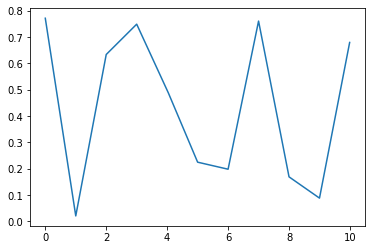
\includegraphics[scale=.5]{linearinterpo}
				\captionof{figure}{Example of Perlin noise using linear interpolation.}
				\label{fig:perlin_lin}
			\end{minipage}
		
			To smooth out the graph, smooth-step interpolation (\autoref{subsec:interpolation}) can be applied to the input values. This is shown in \lstinline|u = fade(x)|, where \lstinline|fade| is the smooth-step interpolation function. Putting it all together with smooth-step interpolation, Perlin noise can be implemented as shown in \autoref{perlin1d}.
			
			\begin{lstlisting}[label={lst:perlin1d}, language=Python, frame=none, caption={1D Perlin Noise.}, captionpos=b]	
				def noise1d(x):
					X = int(math.floor(x)) & 255
					
					x -= math.floor(x)
					
					u = fade(x)
					
					return lerp(u, lattice1d[X], lattice1d[X+1])
				
				# Smooth-step
				def fade(t):
					# 6t^5 - 15t^4 - 10t^3
					return t * t * t * (t * (t * 6 - 15) + 10)
			\end{lstlisting}
		
			This implementation results in noise such as the one depicted in \autoref{fig:perlin1d}, given \autoref{lst:perlin1duse} as an example usage.
			
			\begin{lstlisting}[label={lst:perlin1duse}, language=Python, frame=none, caption={One dimensional example.}, captionpos=b]
				x_vals = []
				y_vals = []
				
				for x in np.arange(0, 10, 0.01):
					x_vals.append(x)
					y_vals.append(noise1d(x))
				
				plt.plot(x_vals, y_vals)
				plt.show()
			\end{lstlisting}
			
			\begin{minipage}{\textwidth}
				\centering
				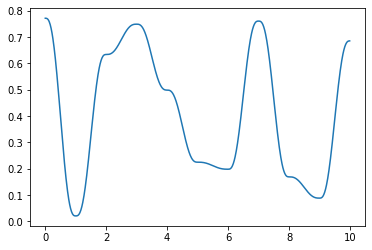
\includegraphics[scale=.5]{smoothnoise}
				\captionof{figure}{One-dimensional Perlin noise.}
				\label{fig:perlin1d}
			\end{minipage} 
	
		\section{2-Dimensional Perlin Noise}
		
			In two-dimensional Perlin noise, the associated lattice is a coordinate grid. The algorithm functions the same as one-dimensional Perlin noise, but instead of two surrounding points and working in a one-dimensional unit, two-dimensional Perlin noise works with four surrounding integer coordinate points, a unit square. Each of the corner points on the unit square now has a two dimensional gradient vector, holding the pseudo-randomly generated values. 
			
			\begin{minipage}{\textwidth}
				\centering
				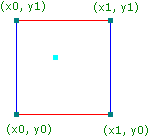
\includegraphics[scale=1.0]{cornergridpoints}
				\captionof{figure}{Arbitrary coordinate (the cyan square), surrounded by integer coordinate points (unit square) \cite{pn-math}.}
				\label{fig:cornergridpoints}
			\end{minipage} 
		
			Given an input of \lstinline|x| and \lstinline|y| variables, four influence values need to be calculated. Given a new two-dimensional coordinate point of \((x,y)\), the same operations must be taken. First, the minimum and maximum bounds must be found for both the \(x\) and \(y\), the same way they were found in one dimension. In \autoref{lst:2d-dst}, these are the \lstinline|X| and \lstinline|Y| variables, holding the minimum \((x,y)\) bounds. The distance from the edges of the unit square are the \lstinline|x| and \lstinline|y| variables. The combination of these four values results in the four corner points of the unit square surrounding the point of interest. The distance vectors are calculated the same way. 
			
			\begin{lstlisting}[label={lst:2d-dst}, language=Python, frame=none, caption={Calculating the distance for two-dimensions.}, captionpos=b]
				X = int(math.floor(x)) & 255   
				Y = int(math.floor(y)) & 255
				
				x -= math.floor(x)
				y -= math.floor(y)
			\end{lstlisting}
		
			\begin{minipage}{\textwidth}
				\centering
				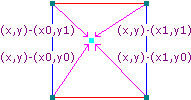
\includegraphics[scale=0.75]{2d_dist}
				\captionof{figure}{Example distance vector calculation \cite{pn-under}.}
				\label{fig:2d_dist}
			\end{minipage} 
		
			Then, the dot product of the distance vectors and their respective gradient vector is calculated. 
			
			\begin{lstlisting}[label={lst:2d-infl}, language=Python, frame=none, caption={Calculating the influence values for two-dimensions.}, captionpos=b]
				s = np.dot(lattice[X    , Y    ], [x    , y    ])
				t = np.dot(lattice[X + 1, Y    ], [1 - x, y    ])
				u = np.dot(lattice[X    , Y + 1], [x    , 1 - y])
				v = np.dot(lattice[x + 1, y + 1], [1 - x, 1 - y])
			\end{lstlisting}
		
			Following this, the influence values must be interpolated. To do this, we can take three linear interpolations, called \emph{bilinear interpolation}. This is shown in \autoref{lst:2d-interp}
			
			\begin{lstlisting}[label={lst:2d-interp}, language=Python, frame=none, caption={Calculating the interpolated final value.}, captionpos=b]
				
				v0 = lerp(s, t, x)
				v1 = lerp(u, v, x)
				
				return lerp(v0, v1, y)
			\end{lstlisting}
		
			By using a hashing function, a dot product of the distance and gradient vectors will also be calculated. Finally, the whole Perlin noise function put together becomes \autoref{lst:2d-perlin}
		
			\begin{lstlisting}[label={lst:2d-perlin}, language=Python, frame=none, caption={Two-dimensional Perlin noise.}, captionpos=b]
				def noise2d(x,y):
					X = int(math.floor(x)) & 255   
					Y = int(math.floor(y)) & 255  
					
					x -= math.floor(x)
					y -= math.floor(y)
					
					u = fade(x)
					v = fade(y)
					
					A = p[X  ]+Y
					B = p[X+1]+Y
					return lerp(v, lerp(u, grad2d(p[A  ], x  , y  ), grad2d(p[B  ], x-1, y  )),
								   lerp(u, grad2d(p[A+1], x  , y-1), grad2d(p[B+1], x-1, y-1)))
			\end{lstlisting}
		
			This will result in an image such as \autoref{fig:lect14-perlin}, where the output values are interpreted as grayscale color values. This implementation's example code is shown in \autoref{lst:perlin2duse}. For retrieving the output of a noise algorithm across a wide area, while a fixed \emph{step-size} is not required, it is the most common method to systematically retrieve the output. A step size is just the distance moved across the lattice with each repetition, in the example, 0.1 in both the \((x,y)\) directions.
			
			\begin{lstlisting}[label={lst:perlin2duse}, language=Python, frame=none, caption={Two dimensional example.}, captionpos=b]
				heightmap = []
				for y in np.arange(0, 10, 0.1):
					for x in np.arange(0, 10, 0.1):
						heightmap.append(noise2d(x,y))
						
				heightmap = np.array(heightmap).reshape((100, 100))
				plt.imshow(heightmap, cmap='gray')
				plt.show()
			\end{lstlisting}
			
			
			
			\begin{minipage}{\textwidth}
				\centering
				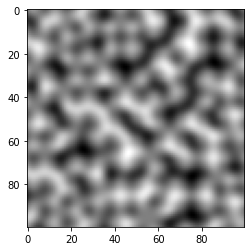
\includegraphics[scale=1.0]{2dperlin}
				\captionof{figure}{Two-dimensional Perlin noise.}
				\label{fig:lect14-perlin}
			\end{minipage} 
		
		\section{3-Dimensional Perlin Noise}
		
			Three dimensional Perlin noise follows the same pattern as one and two dimensional Perlin noise. Instead of for two points, now four points need a distance calculation, and instead of four surrounding points, eight surrounding points must be determined. First, calculate the \((X,Y,Z)\) locations of the unit cube, given input \((x,y,z)\). This calculation is shown in \autoref{lst:3d-perlin}.
			
			\begin{lstlisting}[label={lst:3d-perlin}, language=Python, frame=none, caption={Unit cube calculation.}, captionpos=b]
				# Find unit cube
				X = int(math.floor(x)) & 255
				Y = int(math.floor(y)) & 255
				Z = int(math.floor(z)) & 255
			\end{lstlisting}
			
			Then, the relative position of the coordinate can be found in the unit cube, as well as the smooth-step interpolated coordinate values, shown in \autoref{lst:3d-rel}. 
			
			\begin{lstlisting}[label={lst:3d-rel}, language=Python, frame=none, caption={Relative position calculation of x,y,z coordinates as well as smooth-step interpolation}, captionpos=b]
				# Find relative x,y,z in unit cube
				x -= math.floor(x)
				y -= math.floor(y)
				z -= math.floor(z)
				
				# Compute smooth-step 
				u = fade(x)
				v = fade(y)
				w = fade(z)
			\end{lstlisting}
		
			The next step is to calculate the dot product of the gradient vectors and their respective distance vectors. For three-dimensional Perlin noise, while the original algorithm did involve using random gradients, this caused issues. Instead, in the improved Perlin noise, that amount of randomness is not needed. Instead, unit gradients pointing towards the midpoints of the twelve edges of the cube, shown in \autoref{fig:12}, are used. 
			
			\begin{minipage}{\textwidth}
				\centering
				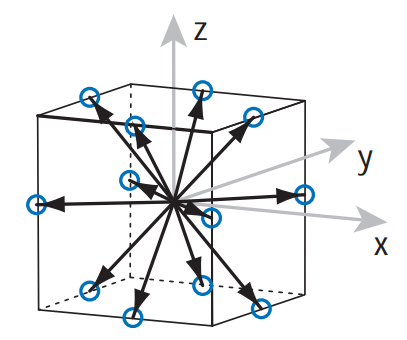
\includegraphics[scale=0.5]{12}
				\captionof{figure}{Improved pseudo-random gradient selection \cite{simplex-demyst}.}
				\label{fig:12}
			\end{minipage}
			
			By randomly selecting one of these values, then doing a dot product with the distance vector, the influence values are obtained. These values are randomly obtained through Perlin's hashing method, discussed in \autoref{subsec:hashing}. The random values resulting from this are the \lstinline|p[]| values. Then \emph{trilinear interpolation} is applied to these influence values, shown in \autoref{label}. Trilinear interpolation is interpolation for three-dimensions, requiring seven total linear interpolations.
			
			\begin{lstlisting}[label={lst:trilinear}, language=Python, frame=none, caption={Tri-linear interpolation of influence values. }, captionpos=b]
				c0 = lerp(u, grad(p[AA  ], x  , y  , z   ), 
							 grad(p[BA  ], x-1, y  , z   ))
				c1 = lerp(u, grad(p[AB  ], x  , y-1, z   ), 
							 grad(p[BB  ], x-1, y-1, z   ))
				
				c2 = lerp(u, grad(p[AA+1], x  , y  , z-1 ), 
							 grad(p[BA+1], x-1, y  , z-1 ))
				c3 = lerp(u, grad(p[AB+1], x  , y-1, z-1 ), 
							 grad(p[BB+1], x-1, y-1, z-1 ))
				
				c00 = lerp(v, c0, c1)
				c01 = lerp(v, c2, c3)
				
				return lerp(w, c00, c01)
			\end{lstlisting}
		
			A simple example of trilinear interpolation between the points, \(c_{000} = 10\), \(c_{100} = 5\), \(c_{001} = 5\), \(c_{101} = 5\), \(c_{010} = 5\), \(c_{110} = 5\), \(c_{011} = 5\) and \(c_{111} = 10\) on the cube shown in \autoref{fig:trilin} when given \(t = (0.3,0.4,0.5)\) would have the steps shown below.
			
			\begin{minipage}{\textwidth}
				\centering
				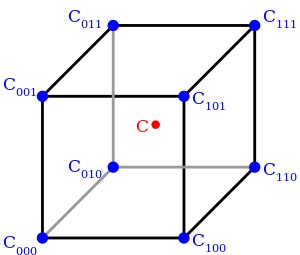
\includegraphics[scale=0.5]{trilin}
				\captionof{figure}{A cube and a point C to trilinearly interpolate the value of. \cite{trilincube}.}
				\label{fig:trilin}
			\end{minipage}
			
			\begin{flalign*}
				c_{00} &= c_{000} + t_\text{x} * (c_{100} - c_{000}) &= 8.5 \\
				c_{01} &= c_{001} + t_\text{x} * (c_{101} - c_{001}) &= 5.0 \\
				c_{10} &= c_{010} + t_\text{x} * (c_{110} - c_{010}) &= 5.0 \\
				c_{11} &= c_{011} + t_\text{x} * (c_{111} - c_{011}) &= 6.5 \\ 
				&&\\
				c_0 &= c_{00} + t_\text{y} * (c_{10} - c_{00}) &= 7.1 \\
				c_1 &= c_{01} + t_\text{y} * (c_{11} - c_{01}) &= 5.6 \\
				&&\\
				c &= c_0 + t_\text{z} * (c_1 - c_0) &= 6.35
			\end{flalign*}
			
			The result of three-dimensional Perlin noise is an image such as the one shown in \autoref{fig:3dscatter}, with a lattice from \([0,10]\) for \((x,y,z)\) and a frequency of \(0.01\). 
			
			\begin{minipage}{\textwidth}
				\centering
				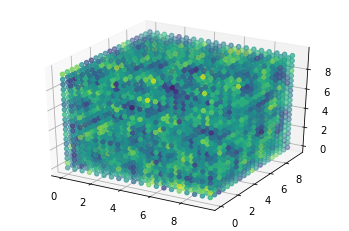
\includegraphics[scale=0.5]{3dperlinscatter}
				\captionof{figure}{Three-dimensional Perlin noise scatter-plot.}
				\label{fig:3dscatter}
			\end{minipage}
			
			While Perlin noise can scale to n-dimensions, it gets more computationally complex for each added dimension. In one dimension, calculations were required for each of the two points surrounding the point in question. In two dimensions, calculations were required for the four points of the unit square. In three, this becomes eight for the unit cube. The number of linear interpolations required for this calculation increased similarly, from one to three to seven. From this, Perlin noise's runtime scaling can be determined - \(O(2^k)\), where \(k = dimensionality\). For example, in \(k=1\) linear interpolation calculation and two surrounding points need to be considered. In two dimensions, \(k=3\) linear interpolations are necessary, and four surrounding points need to be considered. In \(k=3\), seven linear interpolations and eight points are required. This demonstrates a pattern of the number of linear interpolations being equal to \(O(2^{k-1})\), and the number of corner points being equal to \(O(2^k)\). Past three dimensions, Perlin noise's computational complexity becomes more and more impractical.
			
		\section{N-Dimensional Perlin Noise} \label{sec:n-dim}
			
			While Perlin noise saw great success, it was succeeded by algorithms such as Simplex noise, designed to alleviate some of the problems with Perlin noise. This included the computational complexity and the artifacting in the noise created. The artifacting in the noise appears from the necessity for the gradients to pass through zero at the integer coordinates of the lattice. This causes unavoidable artifacting in the noise. In addition, while Perlin noise's computational complexity is acceptable when in three-dimensional space and lower, it suffers greatly from increasing the dimensionality further. Beyond three-dimensional space and its unit cubes, four-dimensional space and beyond's unit cube equivalent is known as a hypercube. The number of corners a hypercube has is \(O(2^k)\), where \(k = dimensionality\). This runtime scaling makes higher dimensions incredibly hard to calculate. 
			
			Simplex noise was designed to be more performant at higher dimensions as well as reducing artifacting that can occur from lattice-based noise. In addition, Simplex noise has a low computational complexity -- O(k\textsuperscript{2}). Simplex noise works based on simplex grids for which it was named after. These grids were constructed by choosing the simplest, repeatable shape to fill a N-dimensional space. Another definition of a n-simplex would be it being the smallest figure that contains \(n+1\) given points in n-dimensional space, while not lying in the space of a lower dimension. In one dimension, this works by choosing repeating line segments, similarly to Perlin noise. In two dimensions, this becomes an equilateral triangle, contrary to the unit square of Perlin noise. In three dimensions, this becomes a trianglular pyramid, also known as a tetrahedron. From four dimensions and onward, this simplex becomes increasingly difficult to visualize. However, there is a pattern in the drawability of simplexes, by creating a new point and connecting it to all previously existing points.
			
			 instead of O(2\textsuperscript{k})\cite{sheet-simplex}
			
			\begin{minipage}{\textwidth}
				\centering
				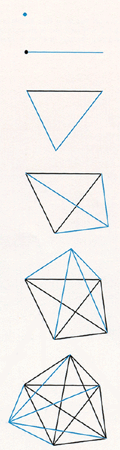
\includegraphics[scale=.75]{six simplexes}
				\captionof{figure}{The first six simplexes \cite{higher-dim-simplexes}}
				\label{fig:fig2}
			\end{minipage}
			
			The relative simplicity of the simplex shape in having as few corners as possible makes it a lot easier to interpolate values in the interior of the shape, relative to the hypercubes used in the original Perlin noise.
			
			In the original Perlin noise function, derivatives were used to compute the gradation between the points. This creates a large increase in computational complexity based on dimensionality. Simplex noise instead uses the summation of kernel values to determine the point's value. To generate the Simplex noise, the value for any point in space must be determined. In two dimensional space, this means skewing the coordinate space along the main diagonal, transforming the squashed equilateral triangles into right-angle isosceles triangles. From there, determining the location is made more simple, as just the integer part of the coordinates is needed for each dimension. Beyond two dimensions, the visualization becomes more difficult, but the steps remain the same.  
			
			\begin{minipage}{\textwidth}
				\centering
				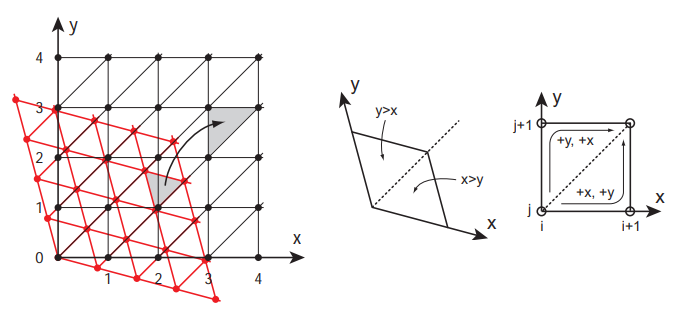
\includegraphics[scale=.5]{skewed grid}
				\captionof{figure}{Skewing a simplex grid in two-dimensional space and determining the cell containing a point. \cite{simplex-demyst}}
				\label{fig:fig9}
			\end{minipage}
			
			The method for interating through a two-dimensional simplex is built around this triangular shape. If the x and y coordinates are known, then all that is needed is to determine which of the two simplices the point lies in. If x > y, the corners become (0,0), (1,0) and (1,1), else the corners are (0,0), (0,1) and (1,1). To traverse this, only one step in the x and one step in the y is needed, but in a different order for each of the simplices. This can then be generalized to any arbitrary amount of N dimensions \cite{simplex-demyst}. While Simplex noise has many advantages over Perlin noise, it has a different visual characteristic, making it difficult to directly replace or compare the two. 
			
			\begin{minipage}{\textwidth}
				\centering
				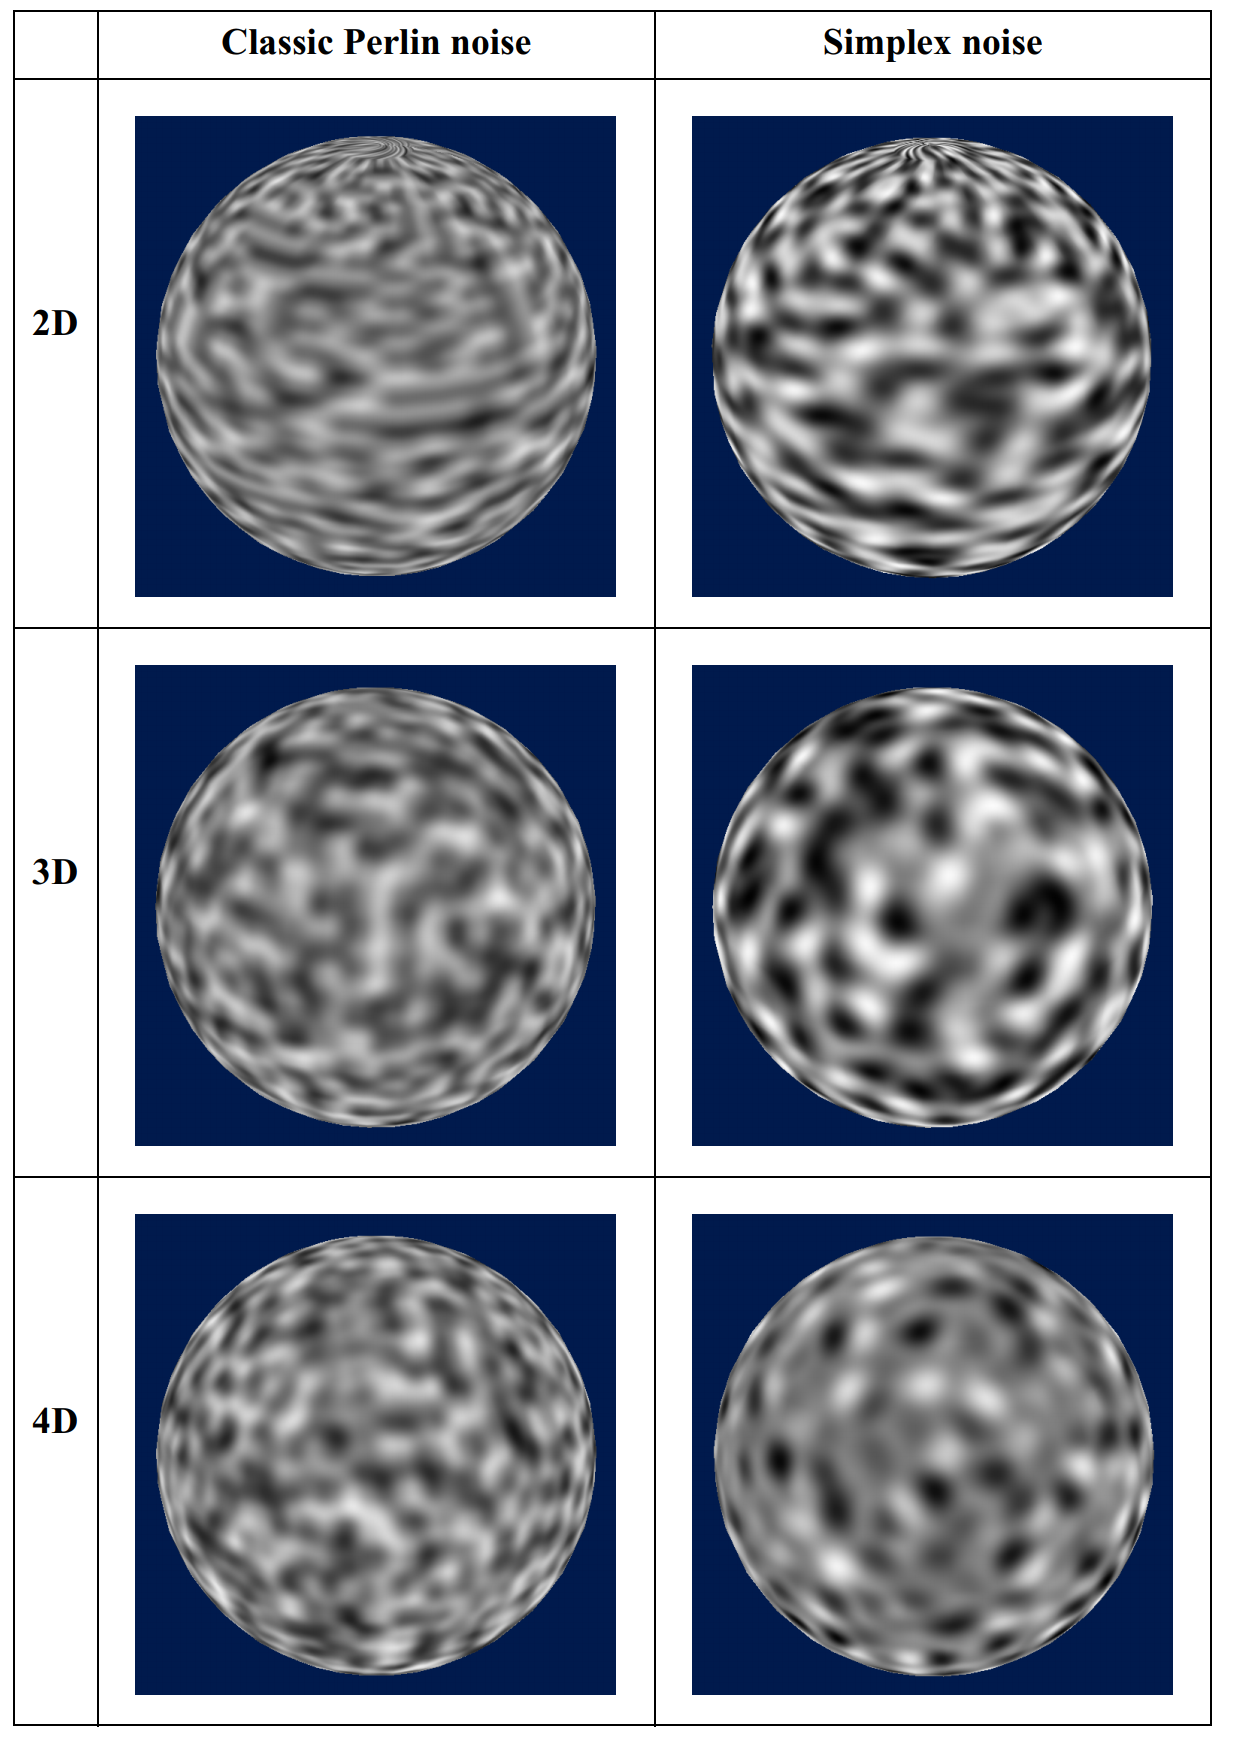
\includegraphics[scale=.2]{perlin vs simplex}
				\captionof{figure}{A comparison of Perlin and Simplex noise \cite{simplex-demyst}}
				\label{fig:fig4}
			\end{minipage}
			
			However, with additional modification using multiple layers or octaves, Simplex noise will run much more computationally efficiently, as well as replicating the visual quirks of Perlin noise.
			
			\section{Layered Perlin Noise}
			To add more diversity, and to increase the range of values given by Perlin noise, \emph{octaves} can be added. The term octave is borrowed from music, where a musical tone that is one octave higher than the previous tone has double the \emph{frequency}. Frequency refers to the number of steps taken between each lattice point. In Perlin noise, this frequency relationship is typically preserved, with increasing octaves of Perlin noise having double the frequency. In simpler terms, the frequency of Perlin noise determines the number of steps taken in total. Some additional terms for octaves in Perlin noise include amplitude, which refers to the range of output values that are possible, as well as the persistence, which refers to the influence that the octave has. Adding octaves together will increase detail, but scales runtime linearly \cite{pn-under}.
			
			\begin{minipage}{\textwidth}
				\centering
				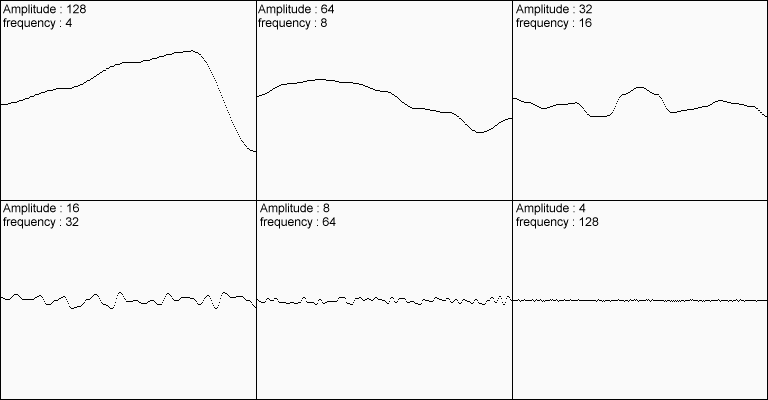
\includegraphics[scale=.4]{octave01}
				\label{fig:oct1}
			\end{minipage}
			\begin{minipage}{\textwidth}
				\centering
				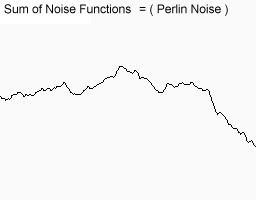
\includegraphics[scale=.75]{octave02}
				\captionof{figure}{Above six figures show noise results with differing amplitudes and frequencies. Below is the sum of the six octaves of Perlin noise \cite{pn-under}.}
				\label{fig:oct2}
			\end{minipage}
		
	\vspace{10pt}
	\let\clearpage\relax
	\chapter{Rendering Methods}
	
		Representing the data generated procedurally is another task with a variety of solutions. Some of these methods include image-based rendering, polygons, and voxels.
	
		\section{Image Based Rendering} \label{sec:imagebasedmethods}
		
		Image based rendering works by rendering based on the screen resolution for the output and the resolution of the input, rather than storing geometric positions. One example of image based rendering is the voxel space rendering system. This rendering system, while named after voxels, has distinct limitations in how it renders, putting it in between two-dimensional and three-dimensional rendering. The voxel space rendering system uses voxel raster graphics to display three-dimensional geometry with low memory and processing requirements. This was developed in the early 90's, involving a height and color map to position the pixels on the screen. While voxel space rendering was not historically used with noise generating algorithms, the rendering system fits the requirements for the use of procedural algorithms such as two-dimensional Perlin noise. By using Perlin noise, the height and color maps can be generated at run-time instead of being created beforehand. An example of this is shown in \autoref{fig:pnvs}. At the time, displaying complex height-maps in three-dimensions was difficult computationally, and voxel space rendering served as a workaround. 
		
		\begin{minipage}{\textwidth}
			\centering
			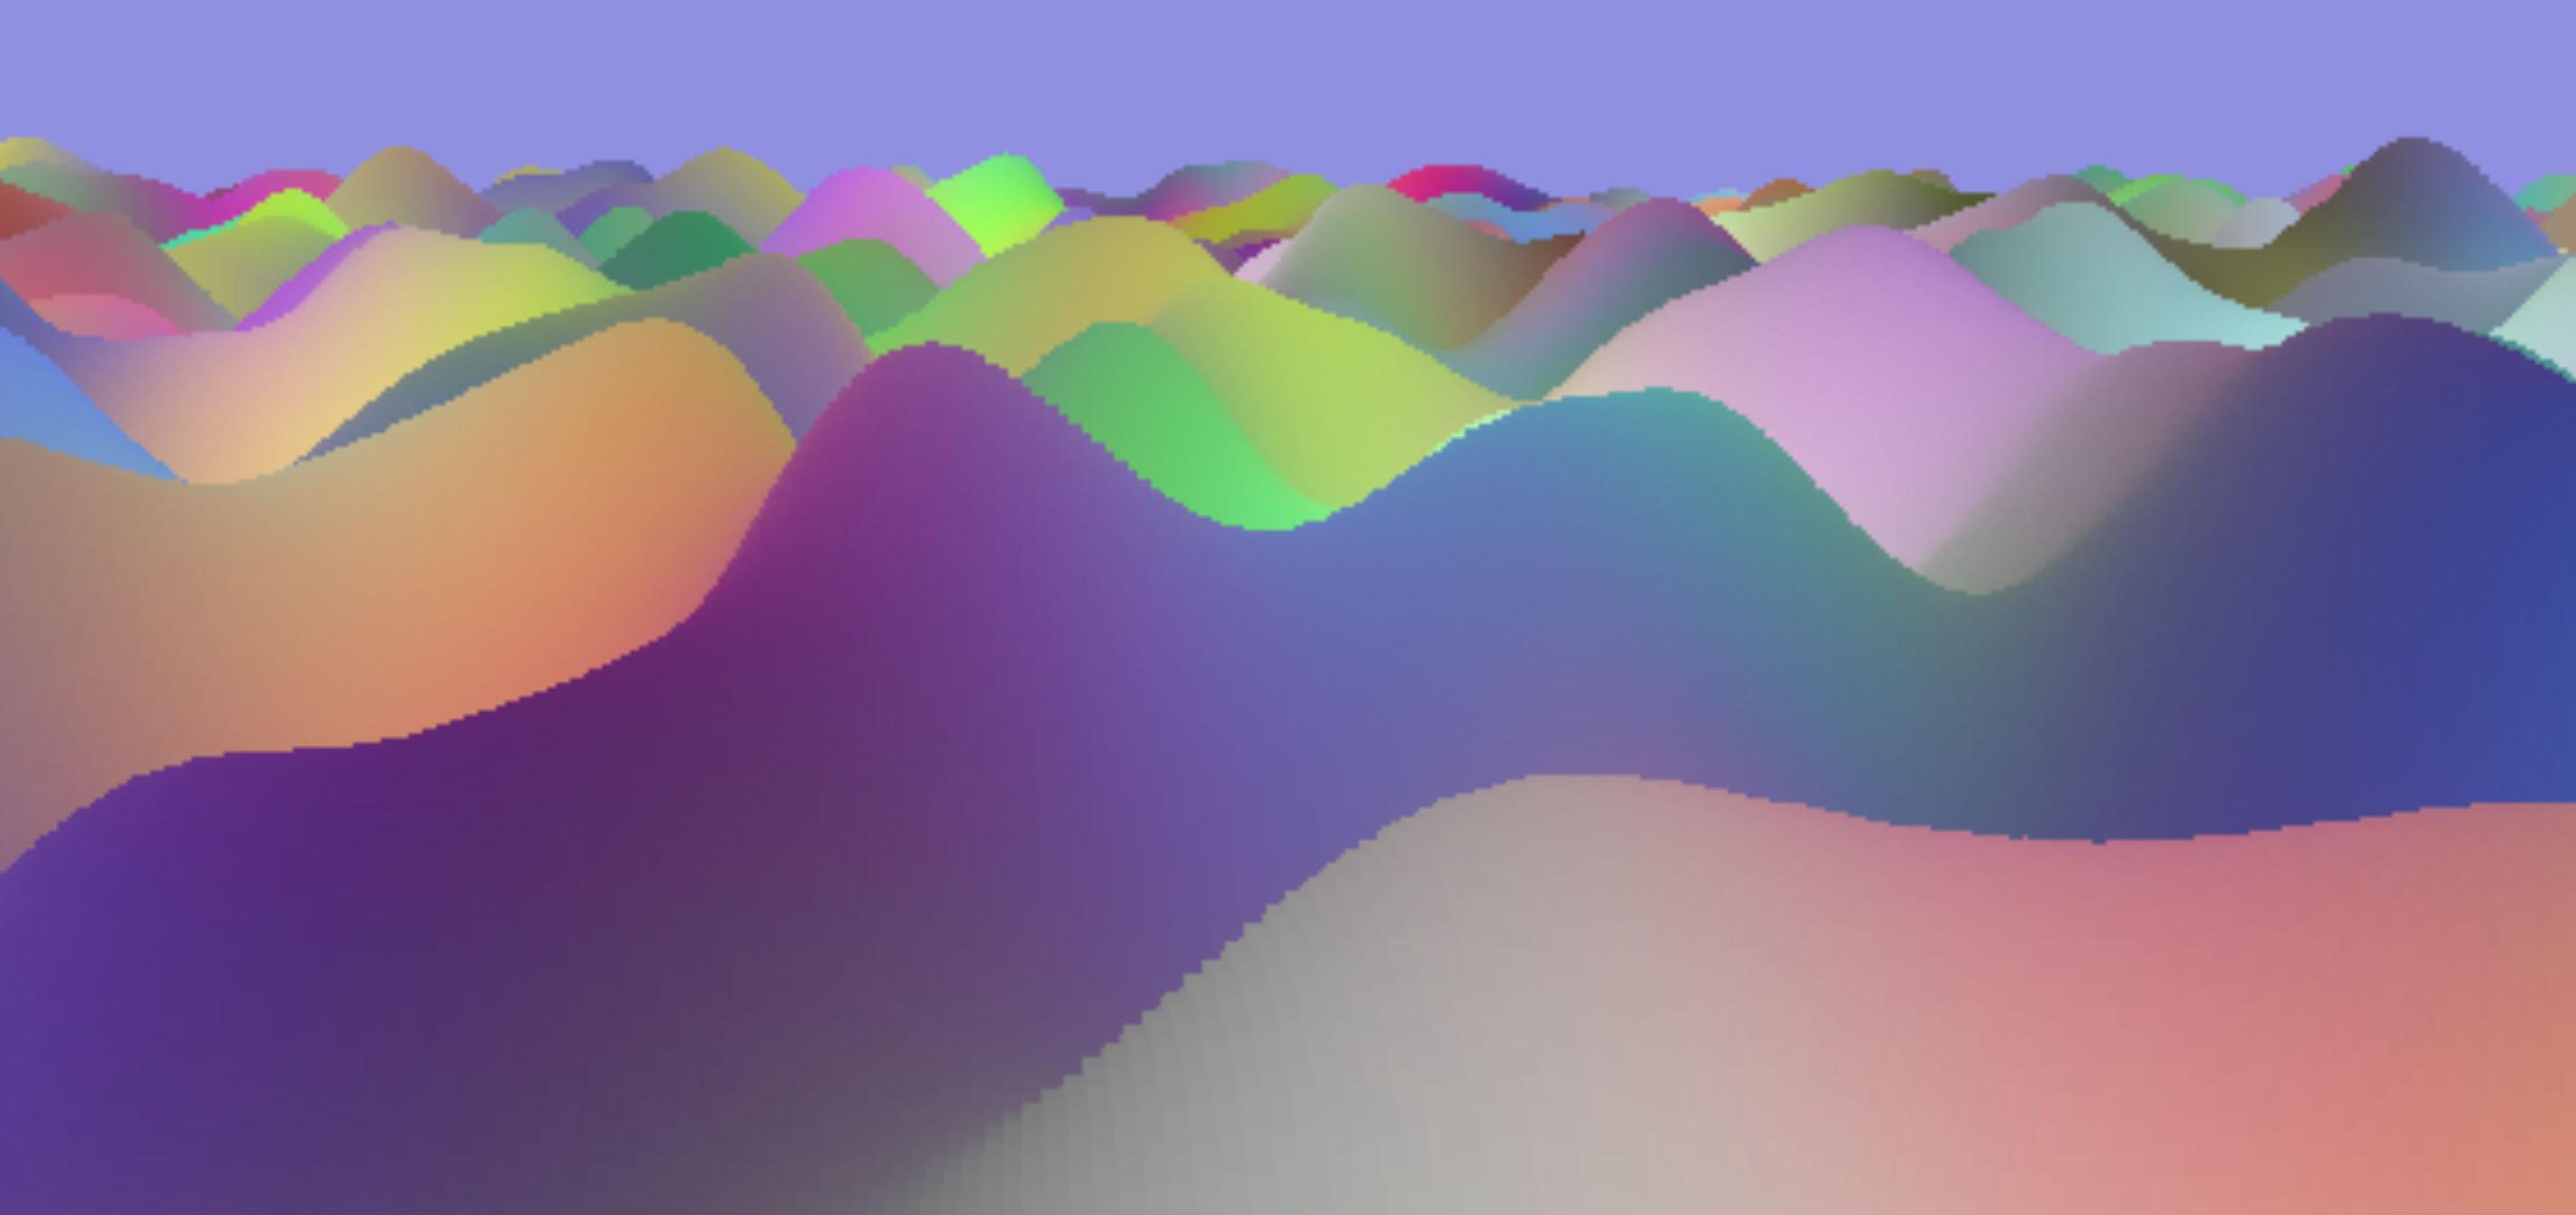
\includegraphics[scale=.15]{proc-voxel}
			\captionof{figure}{Rendering using the Voxel Space engine with a height and color map generated by Perlin noise.}
			\label{fig:pnvs}
		\end{minipage}
		
		The voxel space rendering engine originally utilized a pre-made height and color map to render from. This, combined with a tiling effect and knowledge of the field-of-view of the user's position allowed for a simplified three-dimensional rendering system. Starting from the furthest position to guarantee occlusion, a line on the map is determined in the triangular field of view. This is scaled with perspective projection, and a vertical line is drawn at every point on the screen from the section of the color map. The height of the vertical line is determined from the height drawn from the two-dimensional height map. Then, this is repeated until the entire field-of-view is drawn. This occlusion can be seen in \autoref{fig:vs-raster}. 
		
		\begin{minipage}{\textwidth}
			\centering
			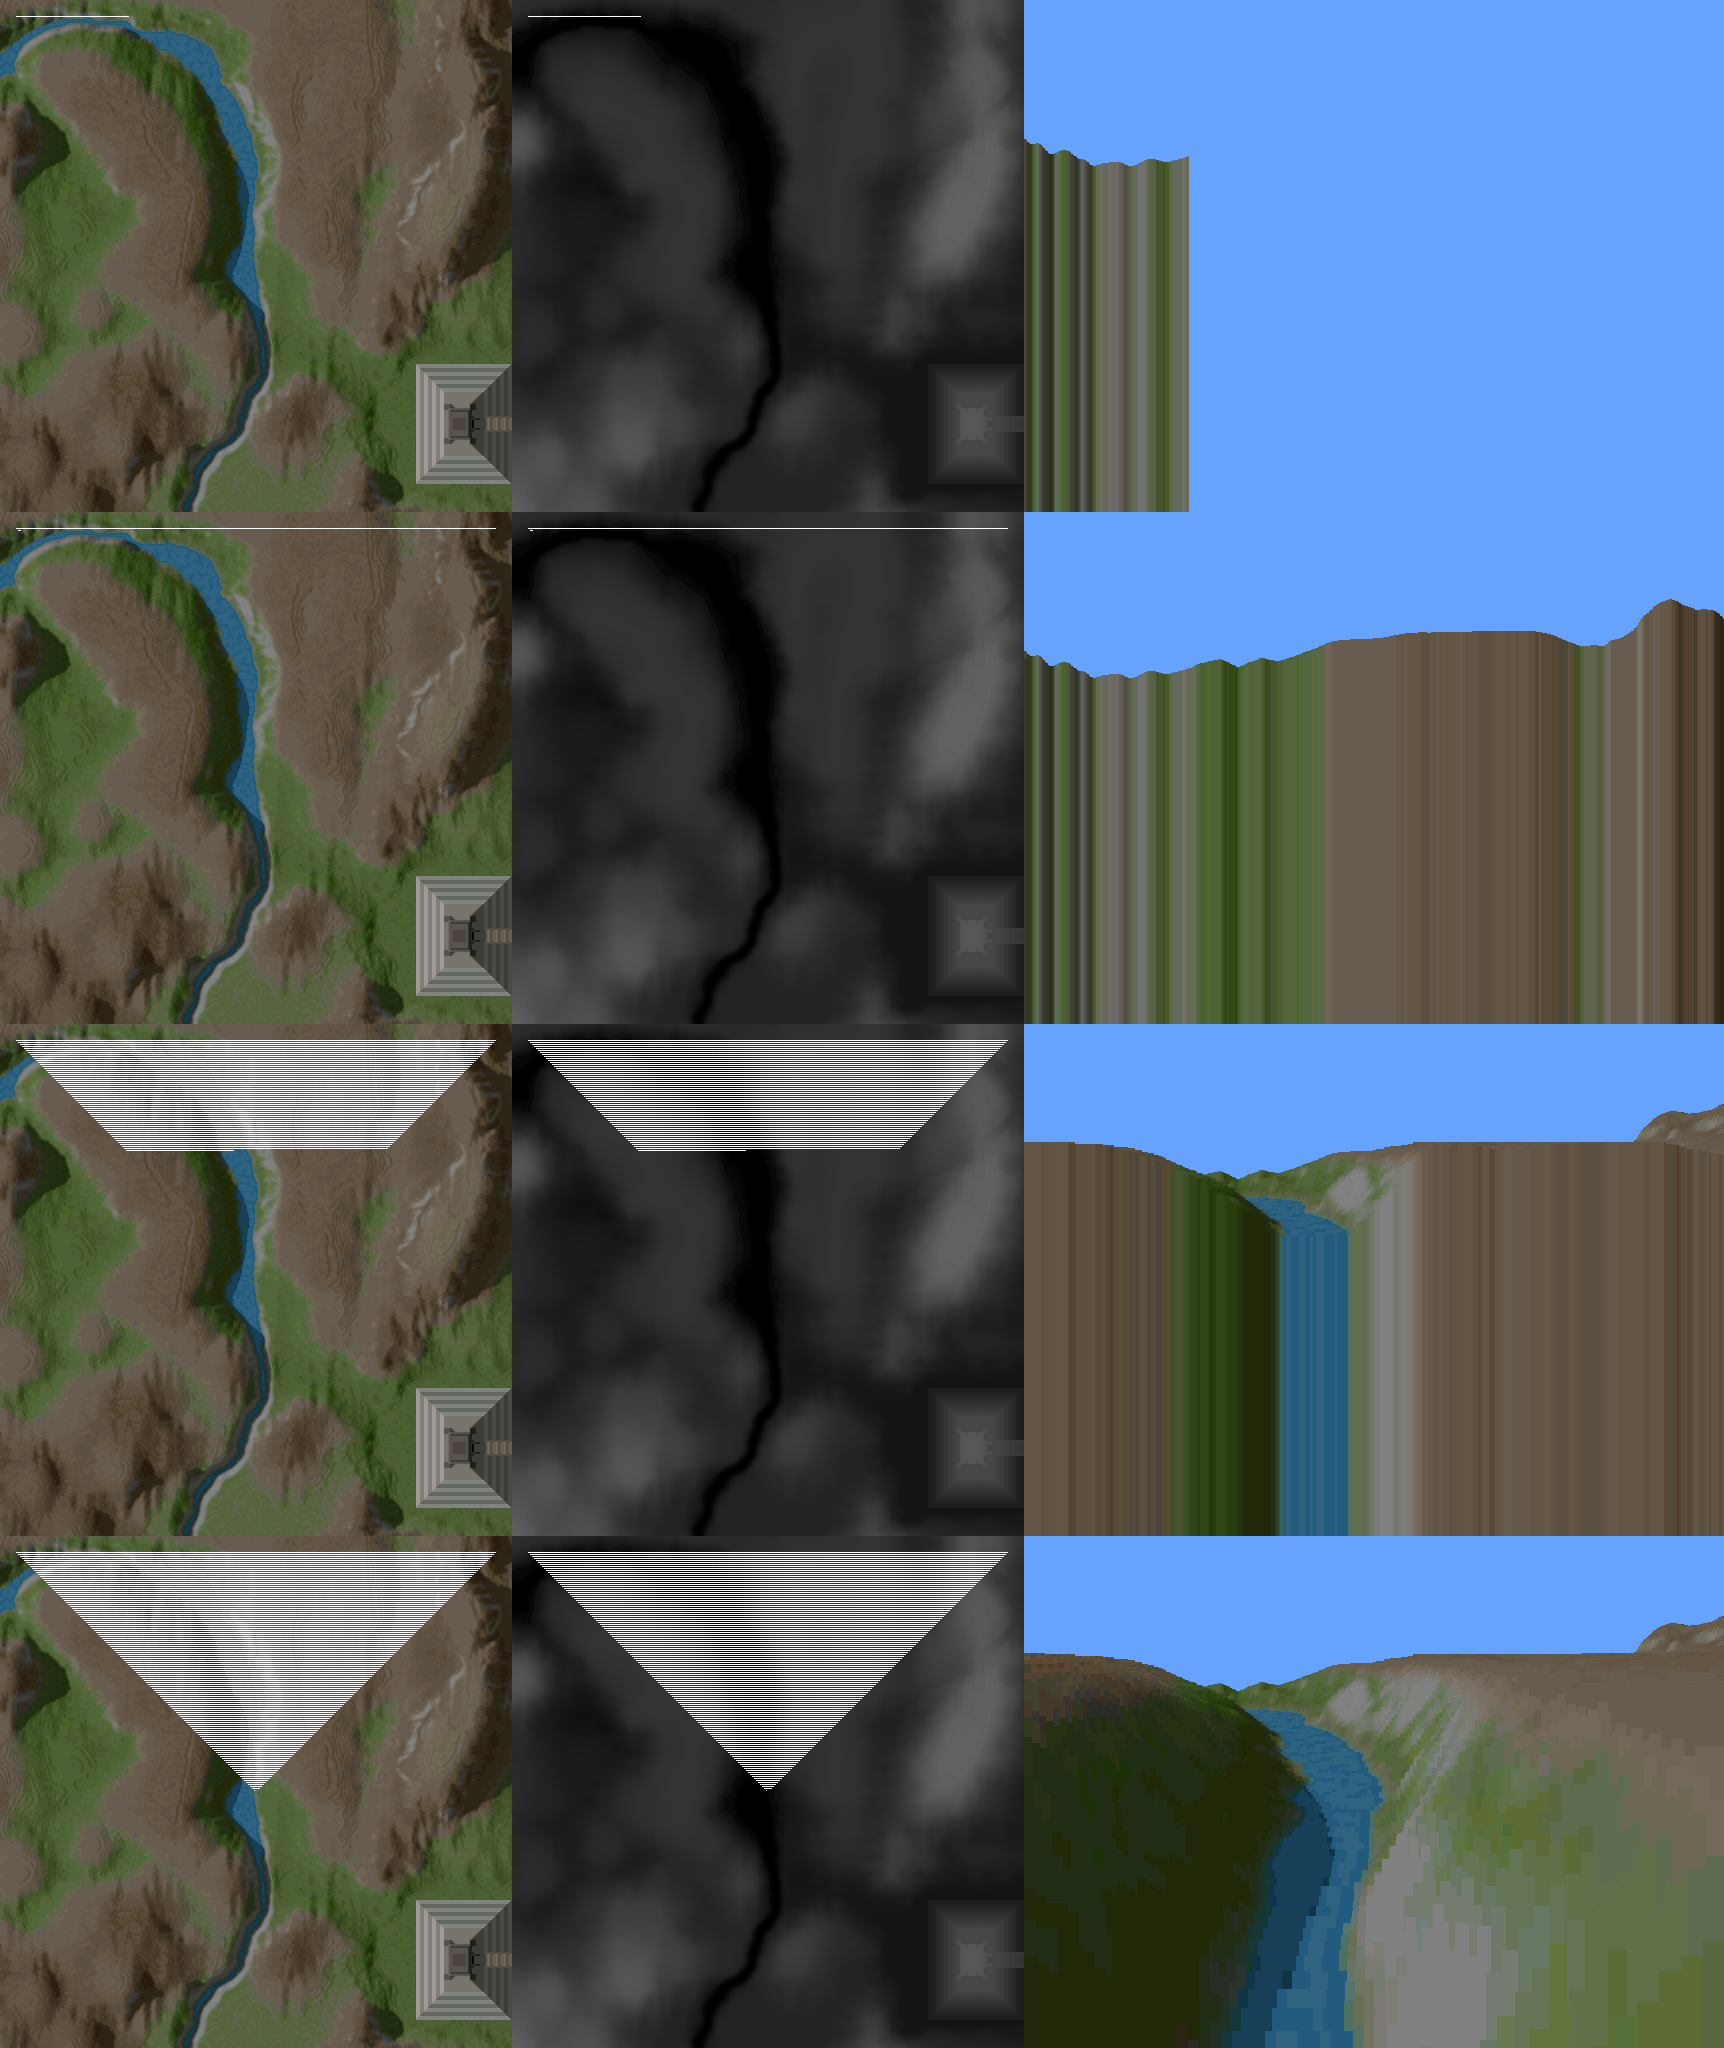
\includegraphics[scale=.2]{line-by-line}
			\captionof{figure}{Basic rasterization of the Voxel Space engine \cite{voxel-space}.}
			\label{fig:vs-raster}
		\end{minipage}
	
		This can be optimized with drawing from front-to-back with the addition of a y-buffer to determine the highest y position to draw. In this case, the y-buffer holds the highest y position, guaranteeing that the closest regions of the height map are displayed properly. However, the voxel-space rendering system has a downside of having fewer pixels to determine the colors and heights of closer landmasses. This creates a pixellated effect for the foreground, while the background is rendered in higher detail. This pixellation and rendering system can be seen in more detail in \autoref{fig:vs-patent}. 
		 
		\begin{minipage}{\textwidth}
		 	\centering
		 	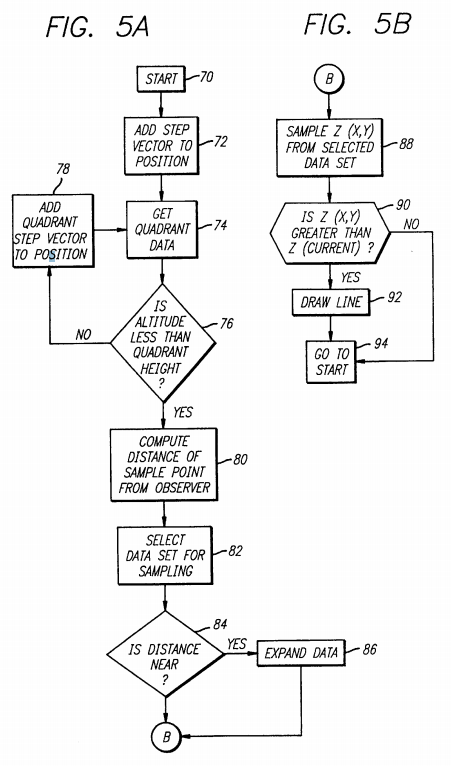
\includegraphics[scale=0.5]{US6020893A}
		 	\captionof{figure}{US Patent 6 020 893 \cite{US6020893}.}
		 	\label{fig:vs-patent}
		\end{minipage}
		
		This weakness can be mitigated in some effect by having multiple heightmaps of differing detail to draw from. This would mitigate some of the advantage of voxel space rendering in increasing the rendering time and processing required for the algorithm. In addition to the weakness in rendering closer objects, height maps are also unable to render more complex geological formations, such as caves, archways or overhangs. Later iterations of the voxel space rendering engine worked around some of these limitations by introducing rendering of both polygons and voxels. Another possible workaround to the low resolution of the voxel space rendering system would be using procedurally generated noise as the platform for creating height maps. By creating the height map dynamically from noise, the memory used for storing the program overall would be smaller, and the resolution would not be constrained, as for areas closer to the camera, the interpolation between the points of the noise map would just be decreased. 
		
		\section{Voxels}
		
		Aside from voxel space rendering, voxels in general represent a volume element in space. Voxels act as a three-dimensional version of a pixel in space. While voxels are typically contained within a cubic cell in three-dimensions, they are not limited to this shape, and can have any number of shapes. These indivudual elements contain its position in space and another parameter or set of parameters, ranging from the color to the material to the texture data, among other possibilities. This allows for easier computation of the absence of terrain data, such as in caves or polygons. In terms of creating a cave, the points in space representing the cave just need to be removed, in contrast to the mapping required to store the vertices in space. 
		
		\label{pt:marching_cubes}
		An example of a structure of representing voxel data is through the marching cubes algorithm. Each voxel (cube) in marching cubes is defined by the pixel values at the corners of the cube. These eight density values each contribute a single value, also known as a density value, with negative values indicating that the point is in empty space, and positive values indicating that the point is inside of solid terrain. A density value of 0, at the boundary of positive and negative, indicates the surface of the terrain. Along this surface is where the polygonal mesh is constructed \cite{marching-cubes}. At any voxel area contained within the eight points, the marching cubes algorithm allows generation of the correct polygons, outputting from zero to five polygons.
		
		To generate the polygons within the cell, the density values must be determined. The set of all corner vertices can be denoted as \(V = {v0,v1,v2,v3,v4,v5,v6,v7}\), where a positive density sets the vertex's bit to one, and a negative density sets the value to zero. 
		
		\begin{minipage}{\textwidth}
			\centering
			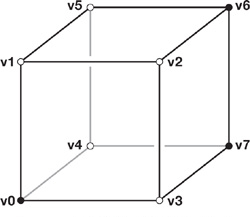
\includegraphics[scale=0.75]{01fig03}
			\captionof{figure}{Interpreting density values from eight voxels into polygonal shapes \cite{marching-cubes}.}
			\label{fig:marching-cube}
		\end{minipage}
		
		\begin{center}
			\begin{tabular}{ l l } 
				\begin{tabular}{ l l }
					Case & = \\
					& = \\
					& = \\
				\end{tabular} 
				&
				\begin{tabular}{ r r r r r r r r }
					{ } v7$\vert$&v6$\vert$&v5$\vert$&v4$\vert$&v3$\vert$&v2$\vert$&v1$\vert$&v0\\
					{ } 1 $\vert$&1$\vert$&0$\vert$&0$\vert$&0$\vert$&0$\vert$&0$\vert$&1\\
					193&&&&&&&
				\end{tabular}
			\end{tabular}
		\end{center}
		
		These bit values can be concatenated with a bitwise OR operation to produce a single byte, in the range of 0-255. Two of these cases end up being trivial -- the concatenated value is 0 or 255, all the points are either inside of a solid terrain, or are in empty space. For the remaining configurations, there are only 14 unique combinations (shown in \autoref{fig:01fig04}) of the remaining 254 possibilities. This allows for the use of a look-up table to generate the polygons \cite{marching-cubes-paul}. 
		
		\begin{minipage}{\textwidth}
			\centering
			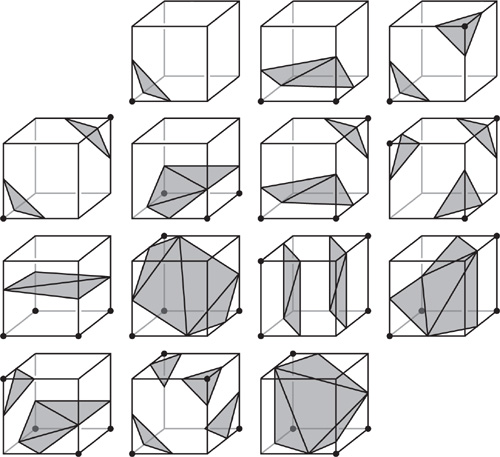
\includegraphics[scale=0.75]{01fig04}
			\captionof{figure}{A single voxel with example density values at the eight corner vertices \cite{marching-cubes}.}
			\label{fig:01fig04}
		\end{minipage}
		
		The placements of the vertices of each of these figures is determined by the density values for each of the corner points, by interpolating the value between these values.	
	
		\section{Polygonal Meshes}
	
		Using a polygonal mesh to represent an object is a common way to representing objects on a computer. A polygon is a planar shape, defined by connecting a series of vertices. A polygon mesh is composed of polygons, and is defined by three parts.
		
		\begin{center}
			\begin{tabular}{ l l } 
				V & a set of vertices (points in space)\\ 
				$E {\subset} (V \times V)$ & a set of edges (line segments)\\ 
				$F {\subset} E$  & a set of faces \\
			\end{tabular}
		\end{center}
		% https://www.classes.cs.uchicago.edu/archive/2015/fall/23700-1/docs/mesh-notes.pdf
	
		These parts allow for the definition of a shape, composed of polygons. Triangles are the default polygon for use in polygonal meshes as three unique points define a plane \cite{polygon}. The flat property of triangles lets the direction that each face of the triangle faces be easy to calculate for -- by contrast, if there is a polygon with a curved surface, then the orientation of the polygon becomes difficult. By connecting the edges of multiple triangles, it is possible to assemble more complex shapes. An example of a polygonal mesh is shown in \autoref{fig:utah-teapot}.
		
		\begin{minipage}{\textwidth}
			\centering
			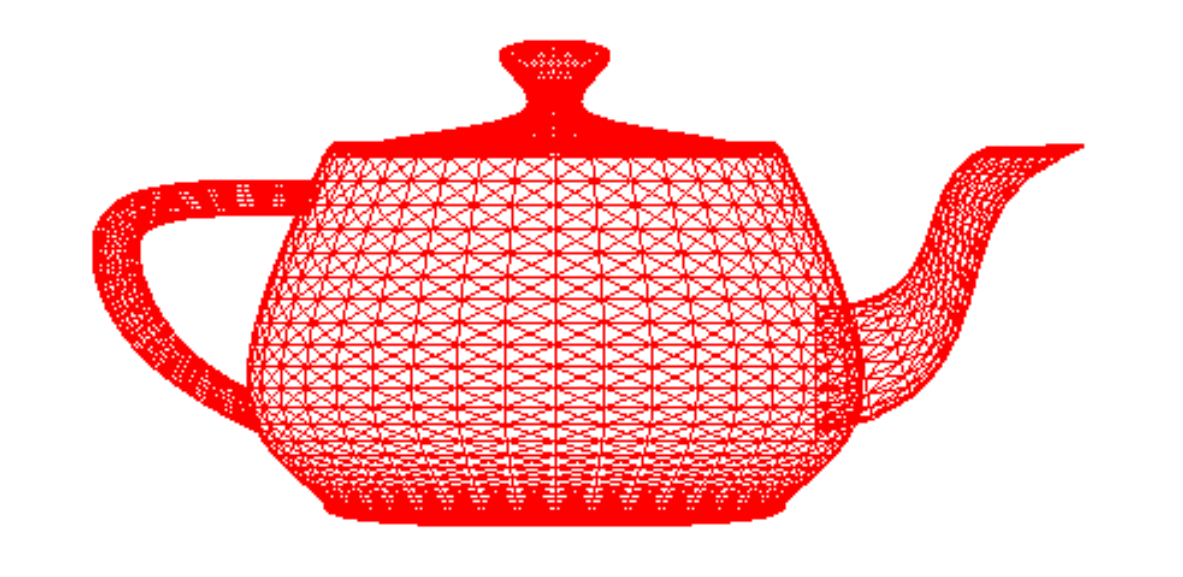
\includegraphics[scale=0.3]{utah-teapot}
			\captionof{figure}{A polygonal mesh of the Utah Teapot \cite{utah-teapot}.}
			\label{fig:utah-teapot}
		\end{minipage}	
	
		A repeating set of triangles cannot capture the appearance of a round edge, but increasing the number of polygons to subdivide the round edge will make it more and more round. Practically, there is a limit to the number of subdivisions that can be calculated for, but there is also a limit to the amount seen at a time. 
		
		
	\vspace{10pt}
	\let\clearpage\relax
	\chapter{Interpretation} \label{chap:interpret}
		
		Rendering data requires some form of interpretation for the data. One form of rendering, voxel-space rendering, relies heavily on the heightmap interpretation of PCG. A \emph{heightmap} interprets the procedurally generated value is taken as a height value. These heightmaps can be rendered in a variety of ways, including using image-based rendering, polygons, or voxels. In \autoref{fig:terrain_mesh}, a heightmap was generated, then another algorithm was used to connect the different vertices together to create a polygonal mesh. 
		
		\begin{minipage}{\textwidth}
			\centering
			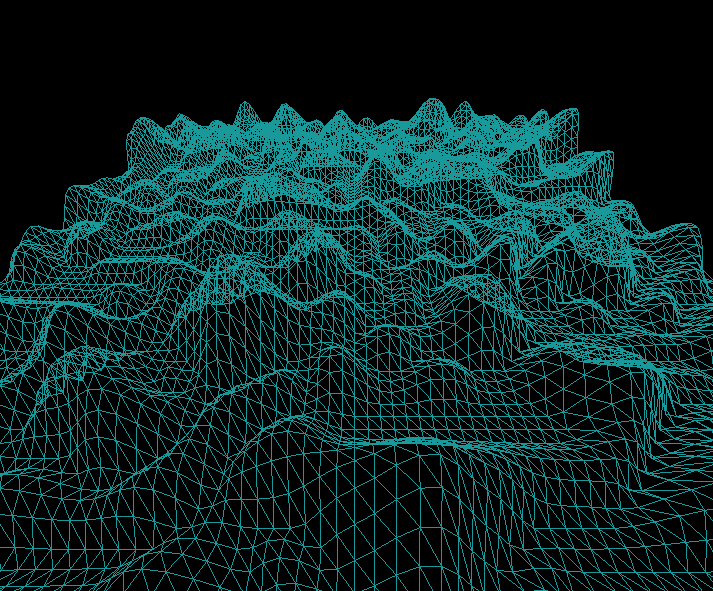
\includegraphics[scale=0.3]{terrain_mesh}
			\captionof{figure}{A heightmap mesh\cite{terrain_mesh}.}
			\label{fig:terrain_mesh}
		\end{minipage}
	
		Another interpretation of data is the interpretation of the procedural values as density values. This particular interpretation is what is used in the Marching Cubes algorithm (see \autoref{pt:marching_cubes}). 
		
		\begin{minipage}{\textwidth}
			\centering
			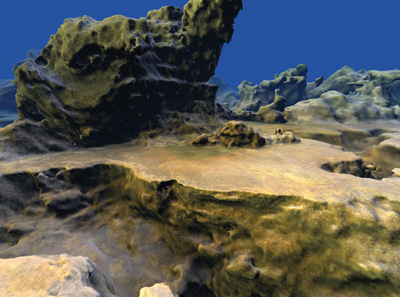
\includegraphics[scale=1.0]{marching}
			\captionof{figure}{Terrain created using the Marching Cubes algorithm\cite{marching-cubes}.}
			\label{fig:marching}
		\end{minipage}
	
		A \emph{texture} is an image or color applied to the surface of a three-dimensional model. For the data created from heightmaps or Marching Cubes, there are also a number of ways to texture this topographical data. One example is similar to the tileset interpretation of procedural data -- just interpret a value, or range of values, as a single color. This often works well for heightmaps, as lower regions can be colored darker, or shaded with water, while higher regions can replicate snowy mountaintops. Another option is tri-planar mapping, which blends three textures to create the least stretched image \cite{triplanar, marching-cubes}. 
		
		Three and four dimensional noise can have uses for PCG as well. For example, one possible application of noise in three dimensions is in the use of generating features such as caves. By setting a limit function, vertain ranges of numbers can be interpreted as empty space. Alternatively, a method such as marching cubes can be used as well. For four dimensional noise, the addition of time as a dimension can be added. While not directly related to topography and geological features, an evolution of terrain over time can be expressed well by using procedural generation -- noise remains relatively constant over time, and flows naturally along each axis. 
		
		While noise has a number of features that make it attractive for PCG of topography, it has a number of downsides as well. Nature expresses many irregularities in landscapes, with smaller features such as boulders and pebbles. These smaller features can be by the use of Perlin noise's smoothing interpolation functions. While this issue can be addressed by modifying the interpolation algorithm, this can create the opposite issue of too much noise. The solution of octaves of noise works to improve this in a way, with the example \autoref{octave02} demonstrating this solution. Another solution to this problem is to just generate features with entirely separate PCG algorithms. In The Witcher 3: Wild Hunt \cite{witcher}, procedural generation is used for the initial creation of the geological formations and terrain, then simulations of nature were applied to generate realistic features \cite{world-machine}. This was then followed by a PCG to dynamically create foliage, based on elevation and the density of other nearby foliage \cite{redengine}, shown in \autoref{fig:vege}. 
		
		\begin{minipage}{\textwidth}
			\centering
			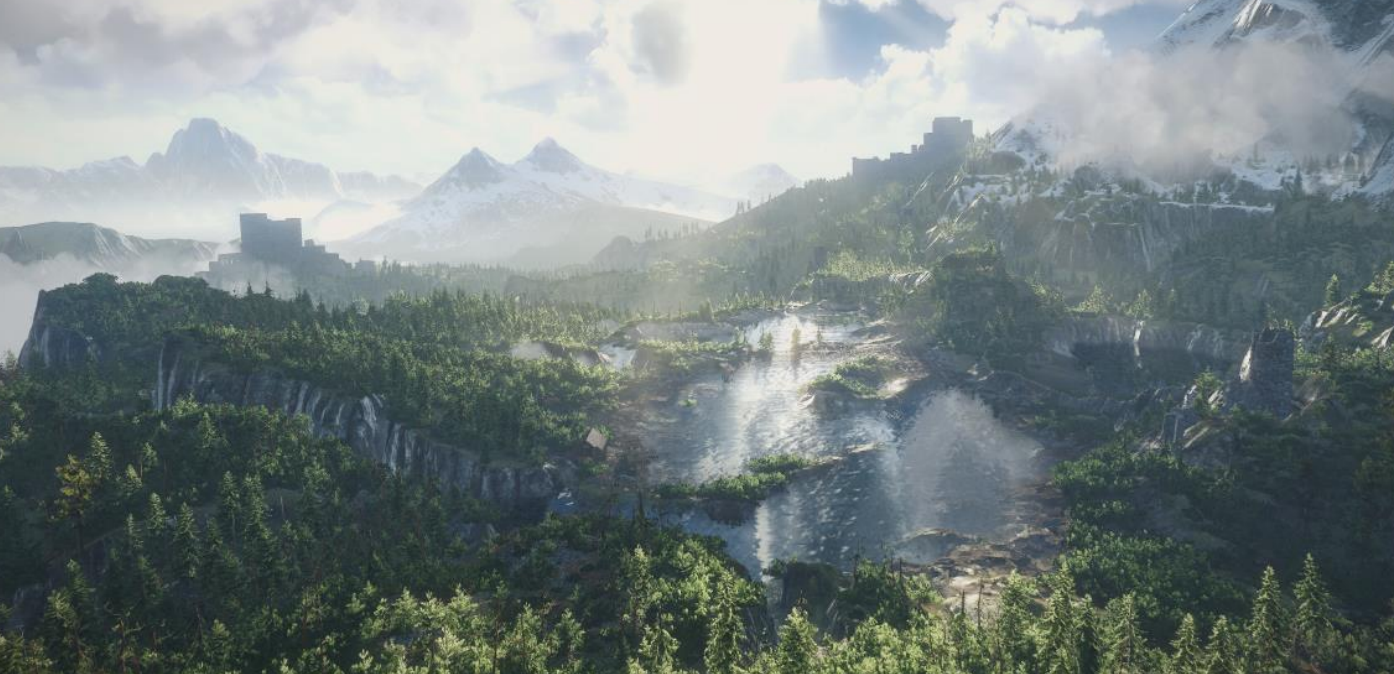
\includegraphics[scale=0.3]{vege}
			\captionof{figure}{Procedural vegetation generation\cite{redengine}.}
			\label{fig:vege}
		\end{minipage}
	
		In the case of generating geological features and topography to emulate real life, which is often a target, geological knowledge is important. For example, in \autoref{fig:simpleisland}, Federico Tomassetti discusses some of the issues with the generated islands, particularly how they do not follow a formation pattern that would be created by plate tectonics. 
		
		\begin{minipage}{\textwidth}
			\centering
			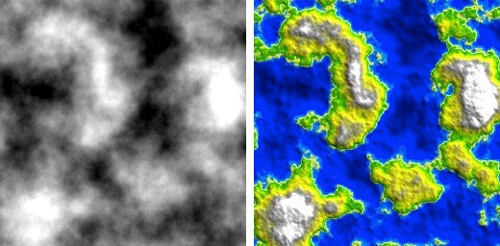
\includegraphics[scale=0.6]{03-simplex-noise-preview-opt}
			\captionof{figure}{Simplex noise island representation\cite{worldd}.}
			\label{fig:simpleisland}
		\end{minipage}
	
		To contrast, \autoref{fig:worldisland} demonstrates similar mountain terrain patterns to a real life satellite map. 
		
		\begin{minipage}{\textwidth}
			\centering
			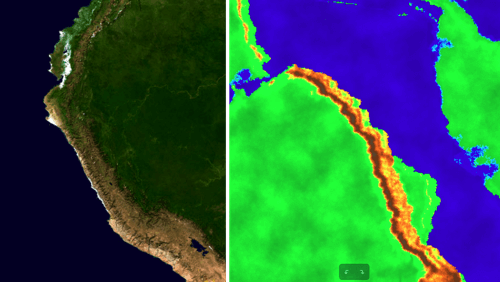
\includegraphics[scale=0.6]{04-worldengine-1-preview-opt}
			\captionof{figure}{Island creation using the WorldEngine\cite{world-machine} tool.\cite{worldd}.}
			\label{fig:worldisland}
		\end{minipage}
	
		The two major considerations for PCG of topography would be: what is the target to create, and how to break up the monotony of PCG. This feature of noise makes it so that, when properly adjusted, it can effectively recreate a target goal, such as the island recreation in \autoref{fig:worldisland}. However, this makes it difficult to adjust for other types of terrain, such as the one shown in \autoref{fig:vege}. As discussed above, noise and other procedural methods are defined by pseudo-randomness in every part of the lattice, generating a sort of monotony from an abundance of information. Since noise differs everywhere, no part of the noise stands out. This increases the significance of landmarks, such as geological formations, to break up the terrain. To effectively build geological formations acting as landmarks into PCG, they must be noticeably unique, as well as not being common. 
	
	\vspace{10pt}
	\let\clearpage\relax
	\chapter{Data Structures} \label{chap:data_structures}
	
		\section{Chunking}
		Between interpreting and displaying the data, storing or reproducing the data is another problem. PCG has the advantage of being able to be recreated through the use of the correct seed and algorithm. For example, to efficiently store the topographical data generated from a procedural algorithm, the topographical data can be broken into smaller pieces. These pieces may be known as \emph{chunks} \cite{tiling}. This compartmentalizes the procedural algorithm. By chunking the data necessary to generate, the amount of noise created at a single time is reduced, or methods such as multi-resolution rendering (see \autoref{fig:voxel-layered-mapping}). This method of chunking can be seen in \autoref{fig:chunks_small}, where a large procedurally generated map is divided into nine visible, or partially visible squares. Each of these squares are generated using their own unique seeds derived from the original seed.
		
		\begin{minipage}{\textwidth}
			\centering
			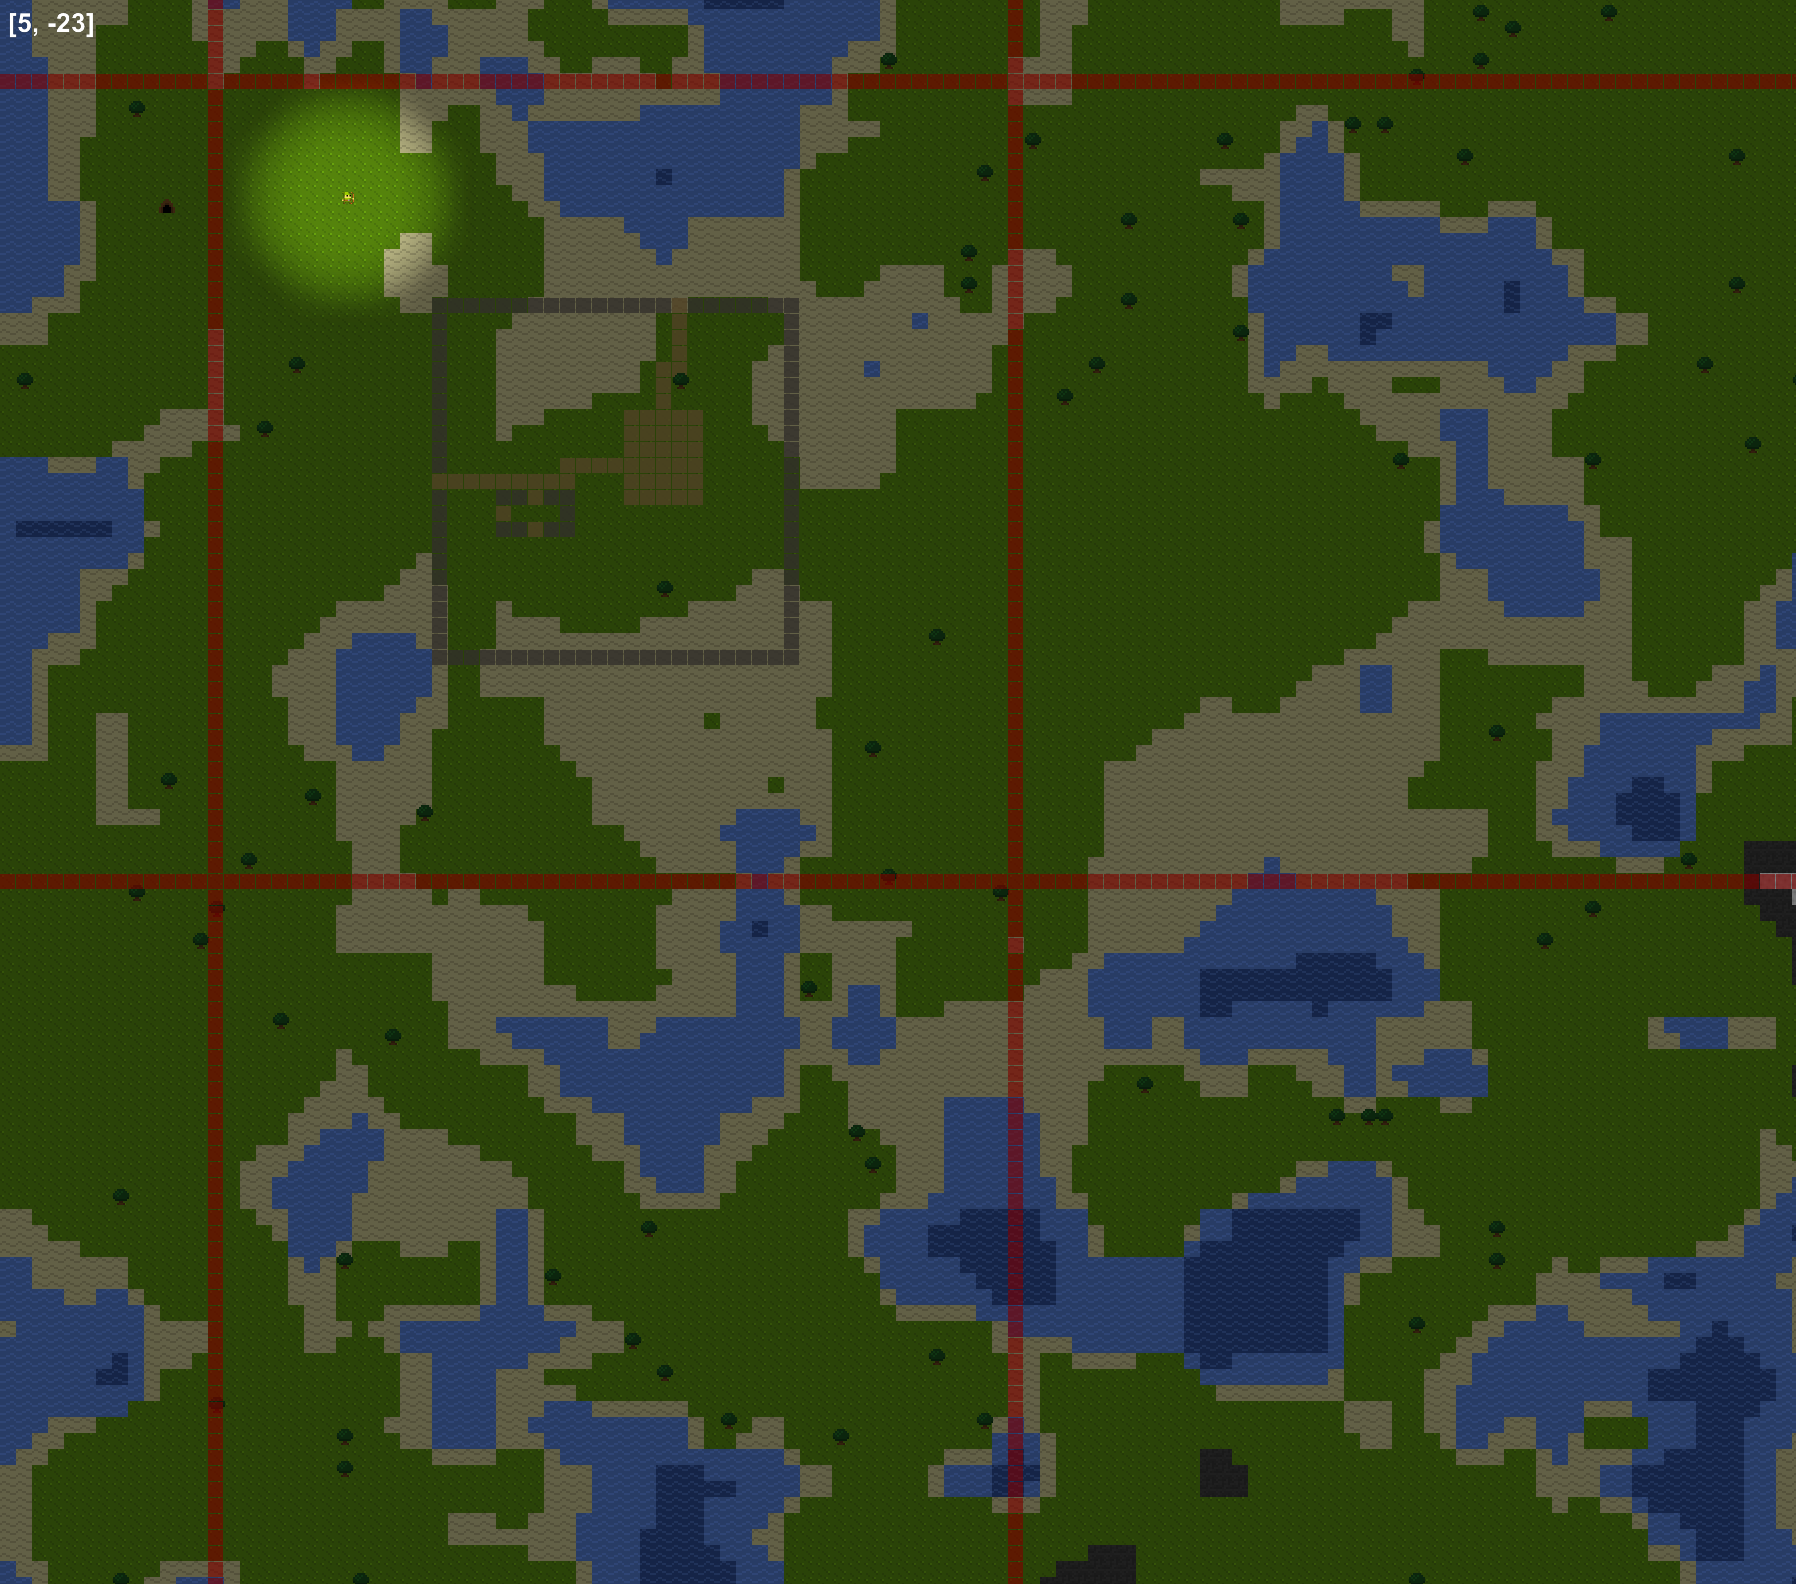
\includegraphics[scale=.4]{chunks_small}
			\captionof{figure}{Chunking a large procedural map. \cite{tiling}}
			\label{fig:chunks_small}
		\end{minipage}
		
		Instead, only the values in the local chunk will be determined. In cases of extremely large-scale topography, where the user may not need or may not see the entire map at the same time, chunking allows for the algorithm to still run. For Perlin noise with multiple octaves and three-dimensional complexity, while memory is not as much of a concern as it was in the past, this helps to alleviate some of the computational strain that can be caused. 
		
		\section{Height Maps}
		
		Another common method of storing topographical data is through the use of height maps. 
		
		\begin{minipage}{\textwidth}
			\centering
			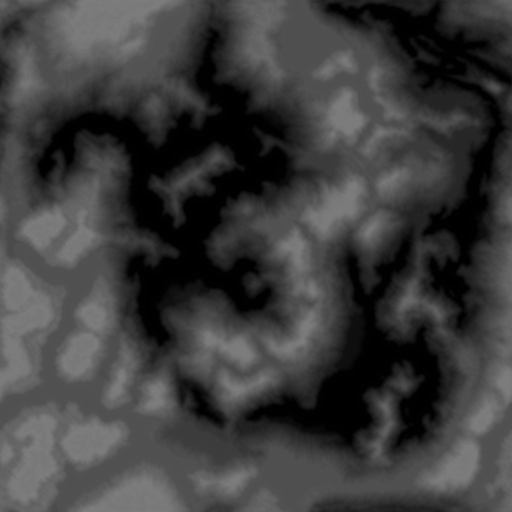
\includegraphics[scale=.4]{D10}
			\captionof{figure}{An example of a height map. \cite{voxel-space}}
			\label{fig:height-map}
		\end{minipage}
		
		The use of height maps is related to the development of some image based rendering and displaying procedural content in two-dimensions. A height map works by storing a single height value at each \((x,y)\) coordinate. This allows for height maps to be stored as an image, as seen in \autoref{fig:height-map}, where the pixel values indicate the height values. Height maps work similarly to topographical maps, with an example of the latter shown in \autoref{fig:top-map}.
		
		\begin{minipage}{\textwidth}
			\centering
			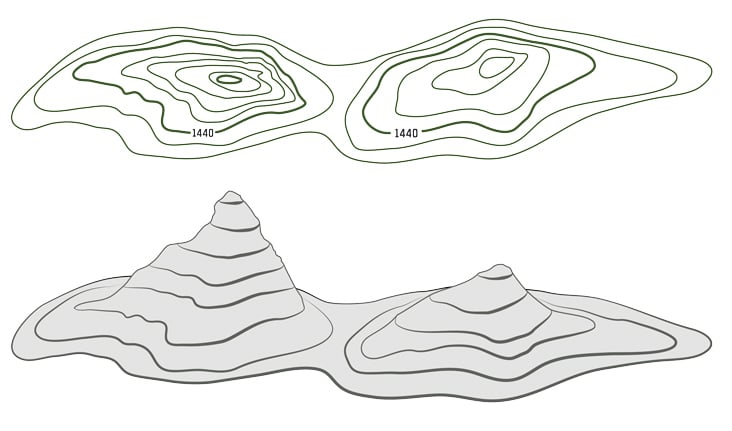
\includegraphics[scale=.4]{top-map}
			\captionof{figure}{A topographical map is shown, with a corresponding three-dimensional representation of the map data below. \cite{top-map}}
			\label{fig:top-map}
	\end{minipage} 
	
	Height maps can be combined with a color map of the same dimensions, in order to map colors to each of the height locations. This effect can be seen in voxel space rendering, shown in \ref{sec:imagebasedmethods} In terms of generating geological formations for landmarking a terrain, height maps add additional limitations on the possibilities. Height maps are unable to store multiple data values at each point, without significant complexity in interpreting the resultant data. This makes the generation of overhangs, arches, or any feature with protruding structures, difficult without additional data storage for these exceptions. A possible solution for this issue includes the storage of overhangs or similar features separately.
		
	\vspace{10pt}
	\let\clearpage\relax
	\chapter{History} \label{chap:development}
		
		\section{Fractals}
		While PCG is entertwined with computational methods, its roots date from before computers. Brownian motion was one of the starting points for procedural algorithms, used to describe the random motion of particles within water. Robert Brown first described this natural phenomenon in 1827. The stochastic process behind Brownian motion was later mapped into an algorithm almost a century later, a method called the Wiener process \cite{inbook}. 
		
		The beginning of the use of fractals to describe landscapes did not coincide with the conception of the term "fractal" by Mandelbrot in the 1970s (see \autoref{sec:fractal}), but developed in the decades to come. This development in capturing surface topography was fueled by Mandelbrot's claim that all forms of nature can only be adequately described using fractals. While the potential of fractals to encapsulate and generate this geometry was noticed in the early 1990s, research at the time was still immature and unable to fully link the processes which create the forms captured by fractals. In terms of general landscapes, fractals were discovered to be able to imitate the self-similarity present in limited regions and limited ranges of scale in real landscapes. Some of the problems in furthering this research included the difficulty in researching and representing the dimensionality of natural terrain \cite{XU1993245}. Generating fractal structures ran into issues with processing time, causing a need for an alternative \cite{inbook}. However, this early PCG found its use in \emph{Star Trek II: The Wrath of Khan} \cite{startrek} to procedurally create imaginary planets. This technology was used later on in an accompaniment to a SIGGRAPH paper to demonstrate more of the ability of fractals. This set the stage for further use in movies such as \emph{The Last Starfighter} and \emph{Return of the Jedi} \cite{ibm-fractal}. 
		
		\section{Cellular Automata}
		
		During the development of fractals, cellular automata also were studied and gained traction. Cellular automata were originally proposed by John von Neumann, focusing on their structure in one and two dimensional grids. This idea was eventually extended into games by John Conway, with the motivation to design a simple set of rules to study the behavior of a population. By tuning different configurations, the "Game of Life" demonstrated a variety of growth patterns stemming from the initial population. Another example of the application of early cellular automata research to games was the \(\sigma(\sigma\textsuperscript{+})\) game, proposed by Sutner. This utilized the capabilities of cellular automata in a 2-d finite grid in order to have two players play against each other \cite{10.1145/349194.349202}.
		
		\section{Noise}
		
		In a similar period, Perlin noise was developed for use in the movie industry as well. It later became a foundation for many other procedural generation algorithms. It was developed in 1983 for use in the sci-fi movie Tron, to map textures onto computer generated surfaces for visual effects. Perlin noise has been used for many visual elements, ranging from the texture creation it was created for to particle effects such as fire, smoke and clouds, as well as landscapes and geological features. It has a variety of uses due to its ability to create a naturalistic appearance \cite{10.1145/325165.325247}.
		
		\section{Applications}
		
		One of the earliest usages of PCG was in Rogue, a video game from 1980 \cite{rogue}. This initial attempt at generating a dungeon in a random manner addressed some of the differences between procedural generation and purely random generation, by introducing some level of control to the designer. Rogue addressed this by using a three by three grid to generate the layout of the level, with hallways randomly connecting the rooms. These rooms would have a variable size to increase the variety of levels producible by the algorithm. This randomized methodology in particular, was created to address the memory constraints of computers at the time, as even with this more mathematical and less memory intensive approach, levels would need to be cleared from memory when moving on to the next one \cite{rogue}.
		
		% can add more here if have time...

		\section{Areas of Research}
	
		More recently, an ongoing area of research for PCG is the introduction of neural networks. One example of this is the procedural generation of terrain via Tensorflow. This implementation was trained on a large data-set of terrain height maps, around 10,000 terrain height maps, with the addition of satellite data to use for coloring. The specific neural network involved in the implementation was a Generative Adversarial network\cite{goodfellow2014generative}, which works on creating fake images, and attempting to discern between real and fake. By iterating this, the network will get better at both tasks, with the generator learning how to create more and more realistic images. For the problem of coloring the terrain, a style network was used to take two images and blend them to create an output image that looks like the content image, but with the style of the reference image. Style networks are also used in other applications, such as the neural networks trained on recreating photographs in a particular artist's style, shown in \autoref{fig:neural-style}. 
		
		\begin{minipage}{\textwidth}
			\centering
			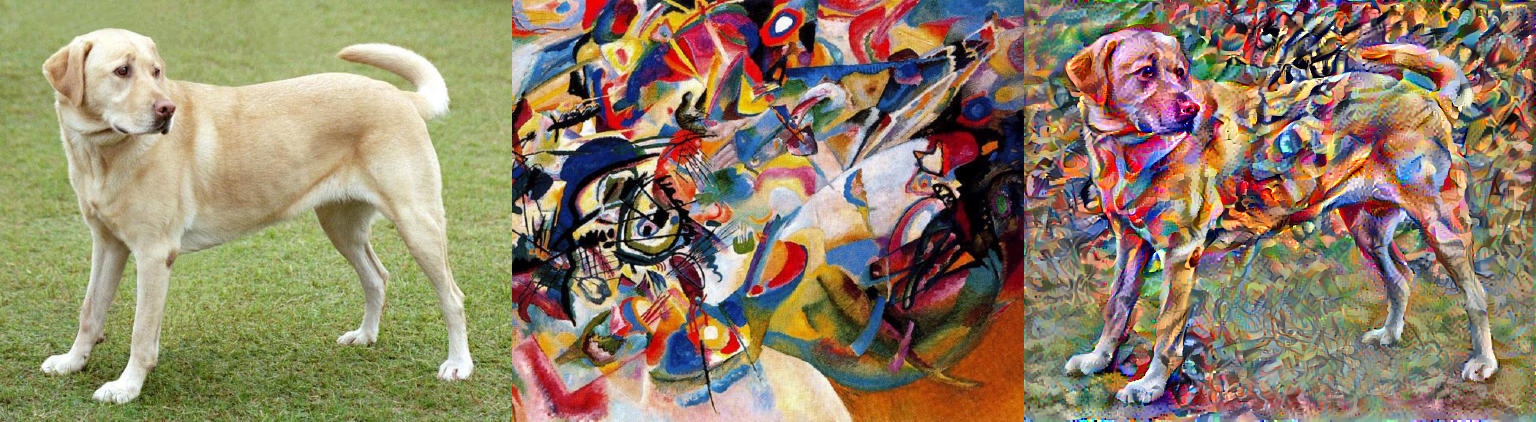
\includegraphics[scale=.3]{stylized-image}
			\captionof{figure}{An example of neural style transfer \cite{tf-style}}
			\label{fig:neural-style}
		\end{minipage}
	
		A kernel is part of image processing, and is applied to an image using convolutions. It is a \(n x n\) matrix, which is multiplied by over the pixels of an image, depending on the stride. \(n\) in this context provides the number of surrounding pixels, in a square formation for which to also draw values from for the new value of the pixel. The stride size refers to the distance the kernel moves for each convolution. If the stride size is too small, this can cause repeated multiplications across the image, a possible cause of artifacting. 
	
		\begin{minipage}{\textwidth}
			\centering
			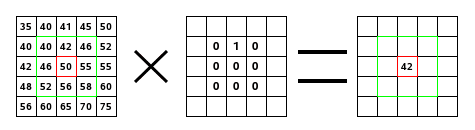
\includegraphics[scale=1]{convolution-calculate}
			\captionof{figure}{An of a kernel (pictured in the center as a 3x3 matrix) being multiplied at the target pixel in red. \cite{gimp}}
			\label{fig:gimp}
		\end{minipage}
		
		The initial processing pipeline for this image based deep learning algorithm utilized convolutional transpose to generate the output height and color-maps. However, this approach led to grid-like artifacting due to the misaligned output size compared to the kernel size. The solution used for combating this was bilinear sampling, by adding pixels from surrounding pixels to determine value rather than the kernels and strides. While the resultant height maps are impressive, additional research is likely required to determine differences between this approach and another approach such as Simplex noise. In \autoref{fig:dl-noise}, the results can be seen. 
		
		\begin{minipage}{\textwidth}
			\centering
			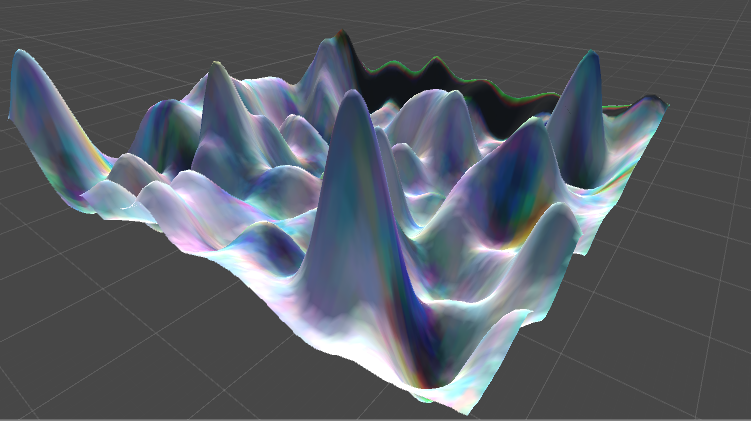
\includegraphics[scale=.3]{rolling}
			\captionof{figure}{Example of three-dimensional worlds created with deep learning \cite{nn-noise}}
			\label{fig:dl-noise}
		\end{minipage}
	
		The field of procedural content generation using machine learning is constantly evolving, as there are many different methodologies that have been applied to this task. The multitude of neural architectures allows for the tailoring of neural networks to different types of generated content, at the cost of necessitating large amounts of searching for the right architectures \cite{Liu_2020}.
		
		In addition to the advancements in noise generation, rendering associated with procedural generation have had advancements as well. For example voxel-based terrain has had advances in both the front and back-end of the algorithms. Voxel-based rendering methods often use a marching cubes algorithm to both smooth voxel surfaces and increase run-times. A modified version of this algorithm was created to facilitate faster implementation and design of a level-of-detail algorithm. Some of the difficulties of this revised implementation of the Marching Cubes algorithm involved finding a suitable compression for the voxel map, as for larger terrains, voxel mapping will quickly grow beyond the limits of addressable memory. In addition, limiting the density of vertices, triangles and individual meshes through a level-of-detail system ensures the higher rendering performance of this revised algorithm. 
		
		The modified Marching Cubes combined with a Transition Cubes algorithm provides a method for stitching together voxel-based meshes and eliminating seams. Rendering the areas of a terrain at different detail layers allows for efficient usage of processing power, but introduces the problem of seams between the cells. This problem can be shown in \autoref{fig:voxel-artifact}. 
		
		\begin{minipage}{\textwidth}
			\centering
			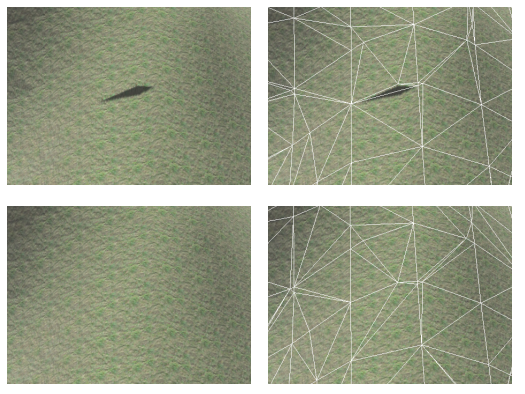
\includegraphics[scale=.75]{voxel-seam}
			\captionof{figure}{A shadow artifact fixed with transition cells \cite{10.5555/1925140}}
			\label{fig:voxel-artifact}
		\end{minipage}
		
		The Transition Cubes method developed in this paper utilizes transition cells inserted in between ordinary cells of a voxel map. This efficiently generates the triangles to connect terrain blocks rendered at different levels of detail, as modifications to one level of detail means that all levels must be adjusted to remain consistent, with the mapping of these different layers shown in \autoref{fig:voxel-layered-mapping}. This technique is known as \emph{multi-resolution rendering}, where objects that need less detail, or are less visible, are rendered at a lower resolution to save on computational power. 
		
		\begin{minipage}{\textwidth}
			\centering
			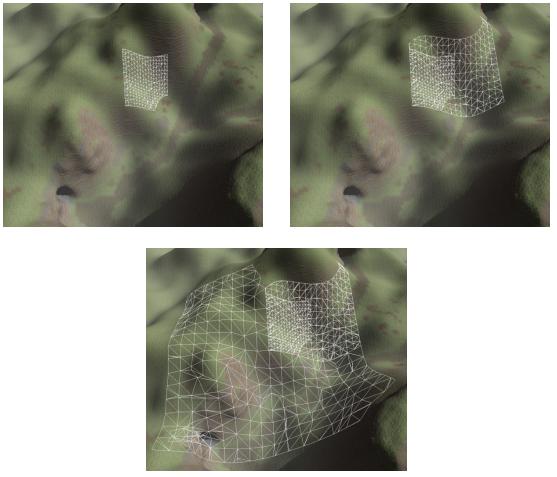
\includegraphics[scale=.75]{voxel-detail}
			\captionof{figure}{Layered resolution details of voxel meshes \cite{10.5555/1925140}}
			\label{fig:voxel-layered-mapping}
		\end{minipage}
		% URL holder http://transvoxel.org/Lengyel-VoxelTerrain.pdf
			
	\vspace{10pt}
	\let\clearpage\relax
	\chapter{Summary}
		
		While procedural generation has a background based in signals processing and fractal mathematics, its usage has extended far beyond these fields. Procedural algorithms are a useful way of automatically generating large amounts of data to interpret. The most well-known noise-based procedural algorithm is Perlin noise, which generates n-dimensional noise from a n-dimensional lattice. Each lattice point has a pseudo-random gradient vector generated, and by finding the dot product of the gradient vector with the associated unit distance vector, the value of the target point can be determined. This is then iterated across the entire range of values that is desired. To store PCG's output, the procedural algorithm can be compartmentalized, or a height map can be created. To then render and interpret the procedurally created data, image based methods, polygonal methods, or voxels are all viable candidates. However, interpreting the result of procedural algorithms, and modifying the outputs to match what is desired is a subjective and long process. Perlin noise and other forms of procedural algorithms have had a long and varied development, with roots in fractal geometry, cellular automata, and signals. 
	
	\newpage
	\renewcommand{\bibname}{References}
	\bibliographystyle{plain}
	\bibliography{refs} % Entries are in the "refs.bib" file
		
\end{document}